%%%%%%%%%%%%%%%%%%%%%%%%%%%%%%%%%%%%%%%%%%%%%%%%%%%%%%%%%%%%%%%%%%%%%%
%%%%%%%%%%%%%%%%%%%%%%%%%%%%%%%%%%%%%%%%%%%%%%%%%%%%%%%%%%%%%%%%%%%%%%
\part{Recursion Theory}\label{part:recursion_theory}\cite{czoo14}
%%%%%%%%%%%%%%%%%%%%%%%%%%%%%%%%%%%%%%%%%%%%%%%%%%%%%%%%%%%%%%%%%%%%%%
%%%%%%%%%%%%%%%%%%%%%%%%%%%%%%%%%%%%%%%%%%%%%%%%%%%%%%%%%%%%%%%%%%%%%%

also \emph{Computability Theory} or \emph{Recursive Function Theory}

\emph{Church-Turing}

Point-free

\fist cf. Combinatory Logic



% ====================================================================
\section{Recursion}\label{sec:recursion}
% ====================================================================

Breaking down to reach a Base Case

Self-referential Functions

\fist Cf. \emph{Process Recursion} (\S\ref{sec:process_recursion})

\fist Cf. \emph{Induction Recursion} (\S\ref{sec:induction_recursion})



% --------------------------------------------------------------------
\subsection{Single Recursion}\label{sec:single_recursion}
% --------------------------------------------------------------------

% --------------------------------------------------------------------
\subsection{Multiple Recursion}\label{sec:multiple_recursion}
% --------------------------------------------------------------------

% --------------------------------------------------------------------
\subsection{Direct Recursion}\label{sec:direct_recursion}
% --------------------------------------------------------------------

% --------------------------------------------------------------------
\subsection{Indirect Recursion}\label{sec:indirect_recursion}
% --------------------------------------------------------------------

(or \emph{Mutual Recursion})

A Set of Mutually Recursive Functions are Primitive Recursive
(\S\ref{sec:primitive_recursive})

Recursive Descent Parser (\S\ref{sec:recursive_descent})

Tree Type (\S\ref{sec:tree_type})



% --------------------------------------------------------------------
\subsection{Structural Recursion}\label{sec:structural_recursion}
% --------------------------------------------------------------------

\emph{Structural Induction} (\S\ref{sec:structural_induction})

Recursive Definition (\S\ref{sec:recursive_definition})

Well-ordering (\S\ref{sec:well_order})

Inductive Type (\S\ref{sec:inductive_type})



% --------------------------------------------------------------------
\subsection{Transfinite Recursion}\label{sec:transfinite_recursion}
% --------------------------------------------------------------------

Transfinite Induction (\S\ref{sec:transfinite_induction})



% --------------------------------------------------------------------
\subsection{Well-founded Recursion}\label{sec:wellfounded_recursion}
% --------------------------------------------------------------------

Well-founded Relation (\S\ref{sec:well_founded})

Well-founded Set (\S\ref{sec:wellfounded_set})



% --------------------------------------------------------------------
\subsection{Non-well-founded Recursion}
\label{sec:nonwellfounded_recursion}
% --------------------------------------------------------------------

\subsubsection{Guarded Recursion}\label{sec:guarded_recursion}

mention \cite{abramsky-gay-nagarajan96} p.12

\cite{atkey-mcbride13}



% ====================================================================
\section{Corecursion}\label{sec:corecursion}
% ====================================================================

Building up from a Base Case

Self-referential Data



% --------------------------------------------------------------------
\subsection{Primitive Corecursion}\label{sec:primitive_corecursion}
% --------------------------------------------------------------------



% ====================================================================
\section{Generative Recursion}\label{sec:generative_recursion}
% ====================================================================

% ====================================================================
\section{Computability}\label{sec:computability}
% ====================================================================

\begin{itemize}
\item Zero-function
\item Successor functions
\item Projection functions
\end{itemize}

Closed under:

\begin{itemize}
\item Composition
\item Primitive Recursion (\S\ref{sec:primitive_recursive})
\item Minimization (\S\ref{sec:mu_recursion})
\end{itemize}

If Minimization is not included, the resulting Functions are Primitive
Recursive Functions that are halting, but do not include all Total
Computable Functions (the Primitive Recursive Functions are a Strict
Subset of the Total $\mu$-recursive Functions).

The Minimization Operator (Unbounded $\mu$-operator) allows for
Unbounded Search and thus the definition of all Computable Functions.



% --------------------------------------------------------------------
\subsection{Decision Problem}\label{sec:decision_problem}
% --------------------------------------------------------------------

% --------------------------------------------------------------------
\subsection{Effective Calculability}\label{sec:effective_method}
% --------------------------------------------------------------------

A \emph{Function} (\S\ref{sec:set_function}) or \emph{Decision
  Problem} (\S\ref{sec:decision_problem}) is \emph{Effectively
  Calculable} if there exists an \emph{Effective Method} for solving
that problem.

An \emph{Effective Method} is a mechanical procedure for solving a
Function or Decision Problem of a specific \emph{Complexity Class}
(\S\ref{sec:complexity_theory}).

See \emph{Computable Function} (\S\ref{sec:computable_function}),
\emph{Computation Models} (\S\ref{sec:computation_model}) and
\emph{Algorithms} (\S\ref{sec:algorithm}).

Effective Topos (\S\ref{sec:effective_topos})



% --------------------------------------------------------------------
\subsection{Divergence}\label{sec:divergence}
% --------------------------------------------------------------------

Computation does not Terminate or Terminates in an (Unobservable)
Exceptional State

Partial Computable Function (\S\ref{sec:partial_computable})

Abstract Rewriting (\S\ref{sec:abstract_rewrite}): Rewrite Convergence
(\S\ref{sec:rewrite_convergence}) if Confluent
(\S\ref{sec:rewrite_confluence}) and Terminating
(\S\ref{sec:rewrite_termination})

Denotational Semantics (\S\ref{sec:denotational_semantics}): $f : A
\cup \{\bot\} \rightarrow B \cup \{\bot\}$ where $\bot$ occurs the
Argument or Function Diverges.

In Process Calculi (\S\ref{sec:process_calculus}): Computation fails
to be Productive (???) %FIXME

Partiality Effect (\S\ref{sec:partiality_effect})



% ====================================================================
\section{Recursively Defined Function}\label{sec:recursive_function}
% ====================================================================

Recursive Definition (\S\ref{sec:recursive_definition})

$\lambda$-recursive, $\mu$-recursive

%FIXME this section is mostly for xrefs

Recursive Functions are defined as Fixed Points
(\S\ref{sec:fixedpoint_combinator}) of regular Functions

in a similar manner (Nested) Data Structures
(\S\ref{sec:data_structure}) can be defined as Fixed Points of regular
Type Constructors (\S\ref{sec:type_constructor})



% --------------------------------------------------------------------
\subsection{Iterative Function}\label{sec:iterative_function}
% --------------------------------------------------------------------

Non-iterative Function (or Linear or Affine ???) %FIXME



% ====================================================================
\section{Computable Function}\label{sec:computable_function}
% ====================================================================

\emph{Computable Number} (\S\ref{sec:computable_real})

\emph{Computable Functions} are the formalized analogues of
\emph{Algorithms} (\S\ref{sec:algorithm}); that is a Function that
is \emph{Effectively Calculable} by an Effective Method
(\S\ref{sec:effective_method}).

\emph{Computable Functions} may be broadly divided into two Classes by
whether they are \emph{Partial} or \emph{Total}. A Total Computable
Function is sometimes called a (Total) \emph{Recursive} or
\emph{Decidable Function}.

There are several equivalent definitions of the class of Computable
Functions, which have reference to different \emph{Models of
  Computation} (\S\ref{sec:computation_model}):
\begin{enumerate}
\item Turing-computable Functions
\item $\mu$-recursive Functions
\item $\lambda$-recursive Functions
\end{enumerate}



% --------------------------------------------------------------------
\subsection{Partial Computable Function}\label{sec:partial_computable}
% --------------------------------------------------------------------

A \emph{Partial Computable Function} (\emph{Partial Recursive
  Function}) is also called \emph{Semidecidable} or \emph{Recursively
  Enumerable} and are the Class of Functions capable of generating
\emph{Recursively Enumerable Sets}
(\S\ref{sec:recursively_enumerable}). A Set, $T$, is
\emph{Co-recursively Enumerable} if the Compliment $\mathbb{N} \ T$ is
Recursively Enumerable.

\emph{Recursively Enumerable} $\mathsf{coRE}$

The Lattice (\S\ref{sec:lattice}) of $\mathsf{RE}$ Sets under
Inclusion is denoted $\mathcal{E}$.

For a Computational Model of Partial Computable Functions see
$\mu$-recursion (\S\ref{sec:mu_recursion}).



\subsubsection{Admissible Numbering}\label{sec:admissible_numbering}

\subsubsection{Markov Algorithm}\label{sec:markov_algorithm}

String Rewriting System (\S\ref{sec:string_rewriting})



% --------------------------------------------------------------------
\subsection{Total Computable Function}\label{sec:total_computable}
% --------------------------------------------------------------------

A \emph{Total Recursive Function} (or \emph{General Recursive
  Function}) is any Total Unbounded $\mu$-recursive Function
(\S\ref{sec:mu_recursion}). \emph{Primitive Recursive Functions}
(\S\ref{sec:primitive_recursive}) are a Strict Subset of General
Recursive Functions.



\subsubsection{Primitive Recursive Function}
\label{sec:primitive_recursive}

The Class of \emph{Primitive Recursive Functions}, $\mathsf{PR}$, are
those given by three Axioms:
\begin{enumerate}
  \item The $0$-ary \emph{Constant Function}, $0$, is Primitive
    Recursive
  \item The $1$-ary \emph{Successor Function}, $S(k) = k + 1$, is
    Primitive Recursive
  \item The $n$-ary \emph{Projection Function}, $P_i^n = k_i$,
    (returning the $i$th argument) is Primitive Recursive
\end{enumerate}
and the Operations:
\begin{enumerate}
  \item \emph{Composition}: Given a $k$-ary function, $f$, and $k$
    $m$-ary Primitive Recursive Functions, $g_1, \ldots, g_k$,
  \item \emph{Primitive Recursion}: Bounded $\mu$-recursion
    (\S\ref{sec:mu_recursion})
\end{enumerate}

Primitive Recursive Functions can be of four types: \cite{kleene52}

\begin{enumerate}
\item Number-theoretic Functions ($\mathbb{N} \rightarrow \mathbb{N}$)
\item Predicates ($\mathbb{N} \rightarrow \{T,F\}$)
\item Propositional Connectives ($\{T,F\} \rightarrow \{T,F\}$)
\item Representing Functions ($\{T,F\} \rightarrow \mathbb{N}$
\end{enumerate}



% --------------------------------------------------------------------
\subsection{Universal Function}\label{sec:universal_function}
% --------------------------------------------------------------------

\emph{UTM Theorem}

$u : \mathbb{N}^2 \rightarrow \mathbb{N}$



% ====================================================================
\section{Semicomputable Function}\label{sec:semicomputable_function}
% ====================================================================

\emph{Upper Semicomputable}

\emph{Lower Semicomputable}

A Partial Function that is both Upper and Lower Semicomputable is just
a Computable Function.



% ====================================================================
\section{Noncomputable Function}\label{sec:noncomputable_function}
% ====================================================================

also \emph{Undecidable Function}

\emph{Algorithmically Unsolvable}

\emph{Turing Degree}

Well-defined (\S\ref{sec:well_defined})



% ====================================================================
\section{Higher-order Function}\label{sec:higherorder_function}
% ====================================================================

\fist See also Combinatory Logic (\S\ref{sec:combinatory_logic}), SKI
Combinator Calculus (\S\ref{sec:ski_calculus})



% ====================================================================
\section{Models of Computation}\label{sec:computation_model}
% ====================================================================

\fist For Models of Concurrent Computation see Process Calculus
(\S\ref{sec:process_calculus}) and Geometry of Interaction
(\S\ref{sec:interaction_geometry})



% --------------------------------------------------------------------
\subsection{$\mu$-recursion}\label{sec:mu_recursion}
% --------------------------------------------------------------------

\emph{$\mu$-recursion} or \emph{Minimization}

\emph{$\mu$-recursive} or \emph{Partially Recursive Functions}

\emph{Bounded $\mu$-recursion}

\emph{Unbounded $\mu$-recursion}



% --------------------------------------------------------------------
\subsection{Turing Machine}
% --------------------------------------------------------------------

See Part \ref{sec:automata_theory} Automata Theory
\S\ref{sec:turing_machine} Turing Machines



\subsubsection{Post-Turing Machine}\label{sec:post_turing}



% --------------------------------------------------------------------
\subsection{Untyped $\lambda$-calculus}\label{sec:untyped_lambda}
% --------------------------------------------------------------------

\emph{Untyped $\lambda$-calculus} describes a Semantics for Computable
Functions (\S\ref{sec:computable_function}).

Untyped $\lambda$-calculus can be seen as a Typed $\lambda$-calculus
with a single Type (\S\ref{sec:type}).

Dana Scott - Set $D$ Isomorphic to Function Space $D \rightarrow D$ of
Functions on itself can be defined if only Continuous Functions are
considered, providing a Model for $\lambda$-calculus. cf. Denotational
Semantics (\S\ref{sec:denotational_semantics})

\fist see also Combinatory Logic (\S\ref{sec:combinatory_logic})

\fist An embedding of $\lambda$-calculus into $\pi$-calculus
(\S\ref{sec:pi_calculus}) is given in Milner92 \cite{milner92}; for an
analogous embedding of Simply-typed $\lambda$-calculus
(\S\ref{sec:simply_typed}) into a Session-typed $\pi$-calculus
(\S\ref{sec:sessiontyped_pi}) see Toninho-Caires-Pfenning12
\cite{caires-pfenning-toninho12}

Interaction Category (\S\ref{sec:interaction_category}) $\cat{SProc}$
(\S\ref{sec:sproc}) of Synchronous Processes is a Model for Typed
$\lambda$-calculus.



\subsubsection{Lambda Expression}\label{sec:lambda_expression}

A \emph{Lambda Expression} is an Expression in the Language of Untyped
$\lambda$-calculus.

The Language of Untyped $\lambda$-calculus consists of the Symbols:
\begin{itemize}
  \item Variables $V = \{ x_1, x_2, \ldots, x_n, \ldots \}$
  \item Abstraction Symbols $\{ \lambda, . \}$
  \item Parentheses $\{ (, ) \}$
\end{itemize}

The Set of Lambda Expressions, $\Lambda$, is defined Inductively:
\begin{enumerate}
  \item $x \in V \Rightarrow x \in \Lambda$
  \item $x \in V \wedge M \in \Lambda \Rightarrow (\lambda x.M) \in
    \Lambda$ (\emph{Abstraction} \S\ref{sec:lambda_abstraction})
  \item $M,N \in \Lambda \Rightarrow (M N) \in \Lambda$
    (\emph{Application} \S\ref{sec:lambda_application})
\end{enumerate}
Notational conventions:
\begin{itemize}
  \item Outermost parentheses may be dropped:
    \[
      (M N) \equiv M N
    \]
  \item Applications are left-associative:
    \[
      M N P \equiv (M N) P
    \]
  \item Body extends as far right as possible:
    \[
      \lambda x.M N \equiv \lambda x.(M N)
    \]
  \item Sequences of Abstractions are contracted:
    \[
      \lambda x.\lambda y.\lambda z.M \equiv
      \lambda xyz.M
    \]
\end{itemize}

A Lambda Expression with no Free Variables is \emph{Closed}, or
sometimes referred to as \emph{Combinators}, equivalent to Terms in
Combinatory Logic (\S\ref{sec:combinatory_logic}).

A Function $f : \mathbb{N} \rightarrow \mathbb{N}$ is a Computable
Function (\S\ref{sec:computable_function}) if and only if there is a
Lambda Expression $F$ such that:
\[
  \forall x,y \in \mathbb{N} (f(x)=y \leftrightarrow F x =_\beta y)
\]



\subsubsection{Lambda Abstraction}\label{sec:lambda_abstraction}

\emph{Lambda Abstraction} is the definition of an \emph{Anonymous
  Function} by the Abstraction Operator $\lambda$ applied to a
Variable (or \emph{Formal Parameter}) $x \in V$ as Binding all Free
occurences of that Variable in the \emph{Body} following the '$.$'
Symbol.

The Variable named by the Lambda Abstraction is \emph{$lambda$-bound}
(or just \emph{Bound}) by the Abstraction.



\paragraph{Free Variable}\label{sec:free_variable}\hfill

A \emph{Free Variable} is one not $\lambda$-bound by a Lambda
Abstraction.

\begin{itemize}
  \item The Free Variables of a Term $x$ consisting of the Variable
    $x$ is just $x$
  \item The Free Variables of $\lambda x.t$ are the Free Variables of
    $t$ without $x$
  \item The Free Variables of $ts$ is the Union of the Free Variables
    of $t$ and the Free Variables of $s$
\end{itemize}

A Free Variable is Bound by its ``nearest'' abstraction:
\[
  \lambda x.y (\lambda x.z x)
\]
The Free occurence of $x$ is Bound by the second Abstraction.



\subsubsection{Lambda Application}\label{sec:lambda_application}

\emph{Application}

The application of a Function $t$ to an Input $s$: $ts$ or $t(s)$



\subsubsection{Lambda Term}\label{sec:lambda_term}

A \emph{Lambda Term} is a Term (\S\ref{sec:term}) in the Language of
Untyped $\lambda$-calculus with the following Inductive definition:
\begin{itemize}
  \item a Variable $x$ is a Lambda Term
  \item for a Lambda Term $t$ and a Variable $x$, the Lambda
    Abstraction $(\lambda x.t)$ is a Lambda Term
  \item for Lambda Terms $t$ and $s$, the Application $(ts)$ is a
    Lambda Term
\end{itemize}
Bracketing may be needed to disambiguate Terms.

By the \emph{Church-Rosser Theorem} (\S\ref{sec:church_rosser}), the
Reduction Rules (\S\ref{sec:reduction_strategy}) of $\lambda$-calculus
are Confluent, so every Lambda Term has at most one Normal Form. In
general there is no Effective method for deciding whether two
arbitrary Lambda Terms are Equivalent.




\subsubsection{Substitution}\label{sec:lambda_substitution}

For a Lambda Term $t$ with Free Variable $x$, a \emph{Substitution}
$t[x/s]$ is the replacement of all occurences of $x$ by a Term $s$.

Substitution is defined uniquiely up to $\alpha$-equivalence
(\S\ref{sec:alpha_conversion}).

\fist See also Substitution (Logic \S\ref{sec:substitution})



\paragraph{Capture-avoiding Substitution}\label{sec:capture_avoiding}\hfill

\emph{Capture-avoiding Substitution}

\emph{Freshness Condition}



\paragraph{Explicit Substitution}\label{sec:explicit_substitution}\hfill



\subsubsection{$\alpha$-conversion}\label{sec:alpha_conversion}

\emph{$\alpha$-conversion} (or \emph{$\alpha$-renaming}) is a renaming
of Bound Variables in a Term that results in an $\alpha$-equivalent
Term:
\[
  \lambda x.x =_\alpha \lambda y.y
\]

\emph{Variable Convention}:
\begin{enumerate}
  \item Bound Variables are distinct from Free Variables
  \item ``Binders'' only Bind Variables not already in Scope % FIXME
\end{enumerate}

When represented as De Bruijn Indices (\S\ref{sec:debruijn_index}),
$\alpha$-equivalent Expressions are Syntactically identical.

\fist See also Nominal Logic (\S\ref{sec:nominal_logic})



\paragraph{De Bruijn Index}\label{sec:debruijn_index}\hfill

\emph{De Bruijn Indices} ``name-free''

Higher-order Abstract Syntax (\S\ref{sec:hoas})



\subsubsection{Contraction}\label{sec:contraction}\cite{seldin03}

Replacement of Subterms:
\begin{enumerate}
  \item $\lambda x . M =_\alpha \lambda y . [y/x]M$
  \item $(\lambda x . M)N =_\beta [N/x]M$
\end{enumerate}



\subsubsection{$\beta$-reduction}\label{sec:beta_reduction}

A \emph{$\beta$-reduction} is a Sequence of Zero or more Contractions
(\S\ref{sec:contraction}). A Term $M$ that Reduces to a Term $N$ is
written $M \rhd N$. $\beta$-reduction may not Terminate but
$\beta$-reduction is Confluent (\S\ref{sec:rewrite_confluence}).

As a Semantics for Functional Programming, a $\beta$-contraction
corresponds to a Computational Step.

Synchronization in Session Calculus (\S\ref{sec:session_calculus})
\cite{orchard-yoshida16}



\subsubsection{$\beta$-conversion}\label{sec:beta_conversion}
\cite{seldin03}

A \emph{$\beta$-conversion} is a Sequence of Zero or more Contractions
or reverse Contractions. A Conversion from Term $M$ to Term $N$ is
denoted $M =_* N$.



\subsubsection{$\eta$-conversion}\label{sec:eta_conversion}

\emph{$\eta$-reduction}:
\[
  \lambda x.y x \rightarrow_\eta y
\]
\emph{$\eta$-abstraction}:
\[
  y \rightarrow_\eta \lambda x.y x
\]

Extensional (\S\ref{sec:extension}) Equivalence of Expressions



\subsubsection{Church Encoding}\label{sec:church_encoding}

\subsubsection{Continuation}\label{sec:continuation}

Abstract Representation (???) of the Control State of a Computer
Program; Reifies the Program Control State

\emph{Continuation Monad}: Computations which can be interrupted and
resumed

Continuation as the ``Future'' of a Computation

Direct Style, Continuation Passing Style (CPS)

Example Identity Function in Direct Style:
\[
  (\lambda x . x) : a \rightarrow a
\]

Example Identity Function in Continuation Passing Style:
\[
  (\lambda x k.k x) : a \rightarrow (a \rightarrow r) \rightarrow r
\]

Cayley's Theorem (\S\ref{sec:cayleys_theorem}): every Group is a
Subgroup of a Canonical Group of Permutations
(\S\ref{sec:permutation_group})

Yoneda Lemma (\S\ref{sec:yoneda_lemma}): every Category is a
Subcategory of a Canonical Functor Category
(\S\ref{sec:functor_category})

Filinski \cite{filinski99}/Piponi: every Monad is a Submonad (???) of
a Canonical Continuation (\S\ref{sec:continuation}) Monad
%FIXME cite piponi, xref submonad



\subsubsection{Deductive $\lambda$-Calclulus}\label{sec:deductive_lambda}

\emph{Intensional Equality} (or \emph{Point-free Equality}): Equal if
$\alpha$-convertible (equality of Function implementations)

\emph{Extensional Equality} (or \emph{Point-wise Equality}): Equal if
Functionally equivalent (perform the same mapping on the same inputs)

Untyped $\lambda$-calculus with Intensional Equality is Inconsistent
as a Deductive System.

Rice's Theorem (\S\ref{sec:rices_theorem})

Von Neumann Universe (\S\ref{sec:vonneumann_universe})



\subsubsection{Evaluation Strategy}\label{sec:evaluation_strategy}

\fist Note that Evaluation Strategies and Reduction Strategies
(\S\ref{sec:reduction_strategy}) are similar but distinct concepts.

Evaluation Function (\S\ref{sec:evaluation_function})

determine when to Evaluate the Arguments of a Function Call
(Operation, Method, Relation, etc.), and what kind of Value to pass
the Function.

Remote Evaluation

Short-circuit Evaluation

In a Typed $\lambda$-calculus (\S\ref{sec:typed_lambda}), a Type
System has Subject Reduction (\S\ref{sec:subject_reduction}) if
Evaluation of Expressions Preserves Types.



\paragraph{Strict Evaluation}\label{sec:strict_evaluation}\hfill

\emph{Eager Evaluation}

Call-by-value \\
Call-by-reference -- Function Application Evaluates the Argument
before proceeding to Evaluation of the Function Body: allows lookup of
the current Value of the Argument as well as modofication via
Assignment



\subparagraph{Call-by-value}\label{sec:call_by_value}\hfill

Applicative Order (or Leftmost Innermost)



\subparagraph{Call-by-reference}\label{sec:call_by_reference}\hfill

(Call-by-address)

Call-by-sharing



\subparagraph{Call-by-copy-restore}\label{sec:call_by_copy_restore}\hfill

(Copy-in Copy-out, Call-by-value-result, Call-by-value-return)

Special case of Call-by-reference



\subparagraph{Partial Evaluation}\label{sec:partial_evaluation}\hfill



\paragraph{Non-strict Evaluation}\label{sec:nonstrict_evaluation}\hfill

\subparagraph{Call-by-need}\label{sec:call_by_need}\hfill

\emph{Lazy Evaluation}

Normal-order (or Leftmost Outermost)

Applicative Simulation (encoding Lazy $\lambda$-calculus into
$\pi$-calculus) \cite{milner92}



\subparagraph{Call-by-name}\label{sec:call_by_name}\hfill



\paragraph{Nondeterministic Evaluation}\hfill
\label{sec:nondeterministic_evaluation}



\subparagraph{Full $\beta$-reduction}\label{sec:full_beta_reduction}\hfill

\subparagraph{Call-by-future}\label{sec:call_by_future}\hfill

\subparagraph{Optimistic Evaluation}\label{sec:optimistic_evaluation}\hfill



\subsubsection{Reduction Strategy}\label{sec:reduction_strategy}

Complex Expression

Simple Expression

\fist Note that Evaluation Strategies
(\S\ref{sec:evaluation_strategy}) and Reduction Strategies are similar
but distinct concepts.

Abstract Reduction (or Rewrite) System (\S\ref{sec:abstract_rewrite})

Reduction Relation (\S\ref{sec:reduction_relation})

Reduction Semantics (\S\ref{sec:reduction_semantics})

$\beta$-reduction (\S\ref{sec:beta_reduction})



\paragraph{Church-Rosser Theorem}\label{sec:church_rosser}\hfill

\paragraph{Call-by-push-value}\label{sec:call_by_pushvalue}\hfill



\subsubsection{Predicate Abstraction}\label{sec:predicate_abstraction}

\emph{Law of Abstraction}



% --------------------------------------------------------------------
\subsection{SKI Combinator Calculus}\label{sec:ski_calculus}
% --------------------------------------------------------------------

Combinatory Logic (\S\ref{sec:combinatory_logic})



% --------------------------------------------------------------------
\subsection{Tag System}\label{sec:tag_system}
% --------------------------------------------------------------------

also \emph{Post Tag Machine}



% --------------------------------------------------------------------
\subsection{Register Machine}\label{sec:register_machine}
% --------------------------------------------------------------------

\subsubsection{Counter Machine}

\subsubsection{Pointer Machine}

\subsubsection{Random Access Machine}

\subsubsection{Random Access Stored Program Machine}



% ====================================================================
\section{Complexity Theory}\label{sec:complexity_theory}
% ====================================================================

Implicit Complexity

Light Affine Lambda Calculus corresponds to the Complexity Class PTIME
%FIXME



% --------------------------------------------------------------------
\subsection{Algorithm}\label{sec:algorithm}
% --------------------------------------------------------------------

An \emph{Algorithm} may be formalized as a sequence of operations that
can be simulated by a Turing-complete system and any Function that is
computable by Algorithm is a Computable Function
(\S\ref{sec:computable_function}).



\subsubsection{Algorithmic Randomness}\label{sec:algorithmic_randomness}



% --------------------------------------------------------------------
\subsection{Function Problem}\label{sec:function_problem}
% --------------------------------------------------------------------

% --------------------------------------------------------------------
\subsection{Communication Complexity}\label{sec:communication_complexity}
% --------------------------------------------------------------------

% --------------------------------------------------------------------
\subsection{Complexity Class}\label{sec:complexity_class}
% --------------------------------------------------------------------

\[
  \mathsf{PR} \subset \mathsf{R} = \mathsf{RE} \cap \mathsf{coRE}
\]



\subsubsection{Double Exponential}\label{sec:double_exponential}

Cylindrical Algebraic Decomposition
(\S\ref{sec:algebraic_decomposition})



% --------------------------------------------------------------------
\subsection{Decidable Set}\label{sec:decidable_set}
% --------------------------------------------------------------------

\emph{Semi-decidable Set}



% --------------------------------------------------------------------
\subsection{Recursive Set}\label{sec:recursive_set}
% --------------------------------------------------------------------

\subsubsection{Recursively Enumerable Set}\label{sec:recursively_enumerable}



% --------------------------------------------------------------------
\subsection{Hyperarithmetic Set}\label{sec:hyperarithmetic_set}
% --------------------------------------------------------------------

\emph{Hyperarithmetic Sets} are the Class of Sets denoted as
$\Delta^1_1$ in the \emph{Analytic Hierarchy}
(\S\ref{sec:analytic_hierarchy}).



% --------------------------------------------------------------------
\subsection{Analytical Set}\label{sec:analytical_set}
% --------------------------------------------------------------------



% --------------------------------------------------------------------
\subsection{Hierarchies}\label{sec:complexity_hierarchy}
% --------------------------------------------------------------------

\[
  \mathsf{AC^0} \subseteq \mathsf{L} \subseteq \mathsf{NC} \subseteq
  \mathsf{P} \subseteq \mathsf{PSPACE} \subseteq \mathsf{EXP}
  \subseteq \mathsf{ALL}
\]

\[
  \Delta_0 = \Sigma_0 = \Pi_0 = \mathsf{R}
\]\[
  \Sigma_1^0 \leftrightarrow \mathsf{RE}
\]\[
  \Pi_1^0 \leftrightarrow \mathsf{coRE}
\]

\emph{$\mathsf{NC}$} is the Class of problems decidable in
Polyalgorithmic Time on a Parallel Computer with a Polynomial number
of Processors.

\emph{Lightface} (no \emph{Set Parameters}) %FIXME explain ``set parameters''
\[
  \Sigma, \Pi, \Delta
\]

\emph{Boldface} (standard hierarchy of Borel Sets)
\[
  \mathbf{\Sigma}, \mathbf{\Pi}, \mathbf{\Delta}
\]

Formulas are considered in \emph{Prenex Normal Form}
(\S\ref{sec:prenex_normal}).
\[
  \Sigma^k_n \cap \Pi^k_n = \Delta^k_n
\]
\begin{itemize}
  \item $k$ is the type of objects being Quantified over with type
    $0 = \mathbb{N}$, and type $i + 1$ are Functions from type $i
    \rightarrow \mathbb{N}$.
  \item $n$ is the number of alternating blocks of Existential and
    Universal Quantifiers
\end{itemize}
The outermost Quantifier block for $\Sigma$ Classes is Existential,
and for $\Pi$ Classes is Universal.



\subsubsection{Arithmetic Hierarchy}\label{sec:arithmetic_hierarchy}

The \emph{Arithmetic Hierarchy} Classifies the Complexity of Formulas
in \emph{First-order Arithmetic}
(\S\ref{sec:firstorder_arithmetic}). The Arithmetic Hierarchy is
extended by the \emph{Hyperarithmetic} and \emph{Analytic
  Hierarchies}.

Every Formula in the Language of First-order Arithmetic is in
$\Sigma^0_n$ or $\Pi^0_n$ for $n \in \mathbb{N}$. Formulas with only
\emph{Bounded Quantifiers} (\S\ref{sec:quantifier}) are in
$\Sigma^0_0$ or $\Pi^0_0$. $\Sigma^0_n$ and $\Pi^0_n$ are defined
Inductively for $n \in \mathbb{N}$:

\begin{itemize}
  \item $\phi = \exists x_1 \exists x_2 \cdots \exists x_k\psi, \psi
    \in \Pi^0_n \rightarrow \phi \in \Sigma^0_{n+1}$
  \item $\phi = \forall x_1 \forall x_2 \cdots \forall x_k\psi, \psi
    \in \Sigma^0_n \rightarrow \phi \in \Pi^0_{n+1}$
\end{itemize}

Thus a $\Sigma^0_n$ Formula begins with Existential Quantifiers and
alternates $n-1$ times between series of Existential and Universal
Quantifiers. The dual is true for $\Pi^0_n$.

By the addition of redundant Quantifiers, a Formula of $\Sigma^0_n$ or
$\Pi^0_n$ is also $\Sigma^0_m$ and $\Pi^0_m$ for $m > n$.

Sets of Natural Numbers that are definable in First-order Arithmetic
are assigned to Classes $\Sigma^0_n$ or $\Pi^0_n$, and to $\Delta^0_n$
if they are both $\Sigma^0_n$ and $\Pi^0_n$.

Turing Computable Sets are at level $\Delta^0_1$.

The \emph{Hyperarithmetic Sets} (\S\ref{sec:hyperarithmetic_set})
are defined as $\Delta^1_1$.

\paragraph{Relativized Arithmetical Hierarchies}\hfill



\subsubsection{Analytic Hierarchy}\label{sec:analytic_hierarchy}

The \emph{Analytic Hierarchy} extends the Arithmetic Hierarchy to
Second-order Formulas. The Classification is of \emph{Analytical Sets}
(\S\ref{sec:analytical_set} of Natural Numbers by the difficulty of
specifying in Second-order Arithmetic
(\S\ref{sec:second_order_arithmetic}), that is Second-order Formulas which
include Quantifiers over $\mathbb{N}$ and Functions from $\mathbb{N}$
to $\mathbb{N}$.

Every Formula in the Language of Second-order Arithmetic is in
$\Sigma^1_n$ or $\Pi^1_n$ for $n \in \mathbb{N}$.

Second-order Arithmetic with no Function Quantifiers:
\[
  \Delta^1_0 = \Sigma^1_0 = \Pi^1_0
\]

Second-order Arithmetic with Existential Function Quantifiers only:
\[
  \Sigma^1_1
\]

Second-order Arithmetic with Universal Function Quantifiers only:
\[
  \Pi^1_1
\]
Both $\Sigma^1_1$ and $\Pi^1_1$ are strictly larger than $\Delta^1_0$.

Second-order Arithmetic with both Existential and Universal Function
Quantifiers-- the class of \emph{Hyperarithmetic Sets}:
\[
  \Delta^1_1 = \Sigma^1_1 \cap \Pi^1_1
\]
is larger than $\Delta^1_0$.

$\Pi^1_1$ Formulas quantified over by Existential Functional
Quantifiers results in the Class $\Sigma^1_2$.

$\Sigma^1_1$ Formulas quantified over by Universal Functional
Quantifiers results in the Class $\Pi^1_2$.

Again, $\Delta^1_2$ is the Intersection of $\Sigma^1_2$ and $\Pi^1_2$
and Inductively this procedure extends to $\Sigma^1_n$, $\Pi^1_n$, and
$\Delta^1_n$.



\subsubsection{Projective Hierarchy}\label{sec:projective_hierarchy}

\emph{Pointclass} (\S\ref{sec:pointclass})

Pointclass of all \emph{Analytic Sets} (\S\ref{sec:analytic_set})
\[
  \mathbf{\Sigma^1_1}
\]

\paragraph{Borel Hierarchy}\hfill



\subsubsection{Counting Hierarchy}

\subsubsection{Exponential Hierarchy}

\subsubsection{Fourier Hierarchy}

\subsubsection{Polynomial Hierarchy}

\paragraph{Pseudo-polynomial}\label{sec:pseudo_polynomial}\hfill

\subsubsection{Polynomial Communication Hierarchy}

\subsubsection{Boolean Hierarchy}




\subsubsection{Blum Complexity Measure}

\emph{Blum Axioms}



% ====================================================================
\section{Hypercomputation}\label{sec:hypercomputation}
% ====================================================================

% --------------------------------------------------------------------
\subsection{Oracle}\label{sec:oracle}
% --------------------------------------------------------------------

% --------------------------------------------------------------------
\subsection{$\alpha$-recursion Theory}\label{sec:alpha_recursion}
% --------------------------------------------------------------------

% --------------------------------------------------------------------
\subsection{Hyperarithmetical Theory}\label{sec:hyperarithmetical_theory}
% --------------------------------------------------------------------



% ====================================================================
\section{Trace Theory}\label{sec:trace_theory}
% ====================================================================

% --------------------------------------------------------------------
\subsection{Trace Monoid}\label{sec:trace_monoid}
% --------------------------------------------------------------------

Free Partially-commutative Monoid

Isomorphic to History Monoids (\S\ref{sec:history_monoid}) and to the
Monoid of Dependency Graphs (\S\ref{sec:dependency_graph})

Free Object (\S\ref{sec:free_object})

$\Sigma^*$ -- Free Monoid (\S\ref{sec:free_monoid}) on Alphabet
(\S\ref{sec:alphabet}) $\Sigma$

A Dependency Relation (\S\ref{sec:dependency_relation}) $D$ Induces an
Independency Relation $I$ on $\Sigma$ defining Sets of Commuting
Letters, which Induces a Binary Relation $\sim$ on $\Sigma^*$ where $u
\sim v$ if and only if there exist $x,y \in \Sigma^*$ and $(a,b) \in
I$ such that:
\begin{align*}
  u &= xaby \\
  v &= xbay
\end{align*}
The Symmetric Transitive Closure of $\sim$ gives an Equivalence
Relation $\equiv_D$ called the \emph{Trace} (\S\ref{sec:trace}) that
Partitions the Free Monoid $\Sigma^*$ into a Set of Equivalence
Classes giving a Quotient Monoid called the \emph{Trace Monoid},
$M(D)$:
\[
  M(D) = \Sigma^*/\equiv_D
\]

Canonical Homomorphism:
\[
  \phi_D : \Sigma^* \rightarrow M(D)
\]
%FIXME universal property

analogous to Free Monoid providing the underpinnings of Formal
Languages (\S\ref{sec:formal_language})

In Concurrent Computation (see Process Calculi
\S\ref{sec:process_calculus}), Commuting Letters are portions of a
``Job'' that can execute Independently of one another and
Non-commuting Letters are Locks, Synchronization Points, or Thread
Joins. %FIXME

\emph{Cancellation Property}

\emph{Dependency Morphism}

Lexicographic Normal Form

Foata Normal Form



\subsubsection{Trace}\label{sec:trace}

A \emph{Trace} $\equiv_D$ is the Transitive Symmetric Closure of the
Binary Relation $\sim$ Induced by Independency Relation $I$ Induced by
the Dependency Relation (\S\ref{sec:dependency_relation}) $D$.

Set of Strings where certain Letters in the String are allowed to
Commute



% --------------------------------------------------------------------
\subsection{Trace Language}\label{sec:trace_language}
% --------------------------------------------------------------------

A \emph{Trace Language} $L$ is a Subset of all Possible Traces $M(D)$
(the Trace Monoid \S\ref{sec:trace_monoid}).

analogous to Free Monoids and Formal Languages
(\S\ref{sec:formal_language})

Trace Closure of a Set of Strings:
\[
  [L]_D = \{[w]_D \mid w \in L\}
\]

Set of Strings in a Set of Traces:
\[
  \bigcup T = \{w \mid [w]_D \in T\}
\]

Trace Language:
\[
  L = \bigcup [L]_D
\]



% --------------------------------------------------------------------
\subsection{History Monoid}\label{sec:history_monoid}
% --------------------------------------------------------------------

Isomorphic to Trace Monoids (\S\ref{sec:trace_monoid}), i.e. Free
Partially-commutative Monoids and to the Monoid of Dependency Graphs
(\S\ref{sec:dependency_graph})

Semi-abelian Categorical Product in $\cat{Mon}$

Histories of Concurrent Processes (see Process Calculus
\S\ref{sec:process_calculus})

Provides a Set of Synchronization Primitives (e.g. Locks, Mutexes,
Thread Joins, etc.) for providing Rendezvous Points between a Set of
Independently Executing Processes (or Threads or Machines).

$A = (\Sigma_1, \ldots, \Sigma_n)$ -- $n$-tuple of Alphabets
$\Sigma_k$

$P(A) = \Sigma_1^* \times \cdots \times \Sigma_n^*$ -- ``Product
Monoid'', all possible combinations of Finite Strings from the
Alphabets %FIXME xref product monoid?

Component-wise Composition:
\begin{align*}
  \vect{u} &= (u_1, \ldots, u_n) \\
  \vect{v} &= (v_1, \ldots, v_n) \\
  \vect{uv} &= (u_1 v_1, \ldots, u_n v_n)
\end{align*}
for all $\vect{u},\vect{v} \in P(A)$A.

$\Sigma = \Sigma_1 \cup \cdots \cup \Sigma_n$ -- Union Alphabet (Set
Union \S\ref{sec:set_union}, not Disjoint Union)

$\pi_k : \Sigma^* \rightarrow \Sigma_k^*$ -- String Projection
(\S\ref{sec:string_projection})

\emph{Distribution}:
\begin{align*}
  & \pi : \Sigma^* \rightarrow P(A) \\
  & \pi(w) \mapsto (\pi_1(w), \ldots, \pi_n(w))
\end{align*}

The Tuple $\pi(a)$ for a Letter $a \in \Sigma$ is called the
\emph{Elementary History} of $a$ giving an Indicator Function
(\S\ref{sec:indicator_function}) for the Inclusion of a Letter $a$ in
an Alphabet $\Sigma_k$:
\[
  \pi(a) = (a_1, \ldots, a_n)
\]
where:
\[
  a_k =
  \begin{cases}
    a \text{if} a \in \Sigma_k \\
    \varepsilon \text{otherwise} \\
  \end{cases}
\]

The \emph{History Monoid} $H(A)$ is the Submonoid
(\S\ref{sec:submonoid}) of the Product Monoid $P(A)$ Generated by the
Elementary Histories.

The Elements of $H(A)$ are called \emph{Global Histories}.

The Projections of a Global History are called \emph{Individual
  Histories}: in Computer Science it is a record of the Sequence of
States of a Process (or Thread or Machine) where the Alphabet
$\Sigma_k$ is the Set of States of the Process.

A Letter that occurs in two or more Alphabets is a
\emph{Synchronization Primitive} between Individual Histories.

The History Monoid $H(\Sigma_1, \ldots, \Sigma_n)$ is Isomorphic to
the Trace Monoid $M(D)$ with Dependency Relation:
\[
  D = (\Sigma_1 \times \Sigma_1) \cup \cdots
    \cup (\Sigma_n \times \Sigma_n)
\]



% ====================================================================
\section{Process Calculus}\label{sec:process_calculus}
% ====================================================================

(or \emph{Process Algebra})

Family of approaches for modelling Concurrent Systems

\begin{itemize}
\item Communicating Sequential Processes (CSP \S\ref{sec:csp})
\item Calculus of Communicating Systems (CSP \S\ref{sec:ccs})
\item $\pi$-calculus (\S\ref{sec:pi_calculus})
\item Chemical Abstract Machine (???)
\item Petri Nets (???)
\end{itemize}

Process Theory (???)

Curry-Howard (\S\ref{sec:curry_howard}) for Process Calculi:
\begin{itemize}
  \item Propositions \emph{as} Session Types (\S\ref{sec:session_type})
  \item Proofs \emph{as} Processes (\S\ref{sec:process})
  \item Cut-elimination (\S\ref{sec:cut_elimination}) \emph{as}
    Communication (\S\ref{sec:communication})
\end{itemize}

Curry-Howard for $\lambda$-calculus identifies a Fragment that is
(Strongly?) Normalizing; Curry-Howard for Concurrency identifies a
Fragment of Process Calculus which is free from Deadlock
(\S\ref{sec:deadlock}): $\pi$-DILL
(\S\ref{sec:sessiontyped_pi}), CP
(\S\ref{sec:classical_processes}), GV (\S\ref{sec:good_variation})

Non-well-founded Set Theory (\S\ref{sec:non_wellfounded}), Systems
(\S\ref{sec:system})


\asterism

Programming Languages:

? -- Scribble

$pi$-calculus (\S\ref{sec:pi_calculus}) -- Pict


\asterism


\cite{winskel-nielsen93}: Atomic Actions over which the Behavior of a
System is Defined %FIXME

Behavior expresses the Patterns of Actions that a System can perform,
capturing aspects such as Deadlock (\S\ref{sec:deadlock}), Mutual
Exclusion (???), Starvation (???), etc.

\fist Note Winskel \& Nielsen \cite{winskel-nielsen93} use the term
\emph{Reactive System} for Distributed (Concurrent) Systems, cf. with
Functional Reactive Programming (\S\ref{sec:frp}).
%FIXME

\[
  \text{Sender} \leftrightarrow \text{Medium}
    \leftrightarrow \text{Receiver}
\]


\textbf{Interleaving}

\emph{Interleaving Model}: Abstracts away Independent Components and
Models Behavior in terms of Sequential Patterns of Actions; Formal
Behavior expressed in terms of Nondeterministic Merging (or
Interleaving) of Sequential Behaviors of Components; e.g. Transition
Systems (\S\ref{sec:state_transition}), Synchronization Trees
(\S\ref{sec:synchronization_tree}), Acceptance Trees (???), Hoare
Traces (???) %FIXME

\emph{Non-interleaving Model}: retains Independent Components in the
Model to allow expression of certain Behavioral Properties such as
Liveness Properties (???); e.g. Petri Nets (???), Event Structures
(???), Mazurkiewicz Traces (???)


\textbf{Nondeterminism}

\emph{Linear-time Model}: Nondeterministic Behavior expressed as Set of
Possible (Determinate) Computation Paths; e.g. Hoare Traces,
Mazurkiewicz Traces, Pratt Pomsets

\emph{Branching-time Model}: e.g. Synchronization and Acceptance
Trees, Petri Nets, Event Structures (CTL$^*$ (\S\ref{sec:ctl_star},
Computation Tree Logic (\S\ref{sec:ctl})


in Interleaving Models, Parallel activities are expressed in terms of
Nondeterminism


\textbf{States vs. Actions}

Explicit Representation of (possibly repeating) States in a System:
e.g. Petri Nets

Abstraction of States in a System, instead focusing on Behavior in
terms of Patterns of occurrences of Actions over Time: Trees, Event
Structures, Traces


Relationships between Behaviors (e.g. Refinement, Component, etc.)
expressed as Moprhisms between Transition Systems

The Inclusion Functor (\S\ref{sec:inclusion_functor}) of
Synchronization Trees (\S\ref{sec:synchronization_tree}) in Transition
Systems is Left-adjoint (\S\ref{sec:adjoint_functor}) to a Functor
``unfolding'' Transition Systems to Synchronization Trees. Ignoring
the Branching of Computation Paths results in Languages
(\S\ref{sec:formal_language}) as Models of Processes (i.e. the Set of
Strings of Actions a Process can perform), and there is also an
Adjoint Inclusion Functor from Languages to Synchronization Trees:
\[
  \text{Languages} \hookrightarrow \text{Synchronization Trees}
    \hookrightarrow \text{Transition Systems}
\]

other Models...

Categories, Operations of Process Calculi as Universal Constructions

certain kinds of Adjunctions (i.e. Reflection
\S\ref{sec:reflection_adjunction} and Coreflection
\S\ref{sec:coreflection_adjunction}) provide a way to express that one
Model is Embedded in (is more Abstract than)


\asterism


Any Proof Reduction or Conversion corresponds to either a Computation
Step or Proces Equivalence \cite{caires-pfenning10}

History Monoid (\S\ref{sec:history_monoid})

Session \S\ref{sec:session}: Sequence of Communications

Linear Logic (\S\ref{sec:linear_logic})

Interaction Categories (\S\ref{sec:interaction_category})


Communication Primitives:
\begin{itemize}
  \item Data Passing (\S\ref{sec:data_passing})
  \item Label Branching (\S\ref{sec:label_branching})
  \item Delegation (\S\ref{sec:delegation})
\end{itemize}


Constructions for Concurrent Programming:
\cite{honda-vasconcelos-kubo98}
\begin{itemize}
  \item Parallel Composition \S\ref{sec:parallel_composition}
  \item Name Hiding \S\ref{sec:name_hiding}
  \item Conditional \S\ref{sec:conditional}
  \item Recursion \S\ref{sec:process_recursion}
\end{itemize}

Inaction $\mono{inact}$ (Unit of $|$)


Session + Recursion $\Rightarrow$ Unbounded Thread of Communications
(\S\ref{sec:unbounded_interaction}) \cite{honda-vasconcelos-kubo98}

Summation-less Asynchronous $\pi$-calculus
(\S\ref{sec:asynchronous_pi_calculus}) \cite{honda-vasconcelos-kubo98}

Asynchronous Polyadic $\pi$-calculus
(\S\ref{sec:polyadic_pi_calculus}) with Branching
\cite{honda-vasconcelos-kubo98}


$\otimes$

$\parr$



% --------------------------------------------------------------------
\subsection{Process}\label{sec:process}
% --------------------------------------------------------------------

\emph{Process}

\emph{Agent}

Terms

Free Names

Free Channels

Free Variables

Free Process Variables

Null Process (\S\ref{sec:null_process})


\asterism


Synchronization Trees (\S\ref{sec:synchronization_tree}) in
Interaction Categories (\S\ref{sec:interaction_category})

$\cat{SProc}$ (\S\ref{sec:sproc}) -- Interaction Category for
Synchronous Processes

$\cat{ASProc}$ (\S\ref{sec:asproc}) -- Interaction Category for
Asynchronous Processes

Processes: ``Relations Extended in Time''

In $\cat{SProc}$, Morphisms are Processes as Labelled Transition
Systems (\S\ref{sec:labelled_transition}) Modulo Strong Bisimulation
(\S\ref{sec:bisimulation})

Non-well-founded Set Theory (\S\ref{sec:non_wellfounded}), Systems
(\S\ref{sec:system})



\subsubsection{Program}\label{sec:program}

A \emph{Program} is a Process with no Free Variables or Free Channels



\subsubsection{Replicated Input Process}
\label{sec:replicated_input_process}

Replicated Input (\S\ref{sec:replicated_input})

$!x(y).P$

\emph{Server} waiting on Channel $x$ to be Invoked
(\S\ref{sec:invocation}) by \emph{Clients}



\paragraph{Invocation}\label{sec:invocation}\hfill

Replicated Input Process $!x(y).P$ (Server)

\emph{Invocation} by Client Spawns a new copy of the Process $P[a/y]$
with $a$ the Name passed by the Client to the Server during the
Invocation



\paragraph{Shared Server}\label{sec:shared_server}\hfill

Session-typed $\pi$-calculus (\S\ref{sec:sessiontyped_pi})

Replicated Server

$!A$ Shared Server for Sessions of Type $A$



\subsubsection{Recursive Process}\label{sec:recursive_process}

Process Recursion (\S\ref{sec:process_recursion})



\paragraph{Variable Agent}\label{sec:variable_agent}\hfill



% --------------------------------------------------------------------
\subsection{Channel}\label{sec:process_channel}
% --------------------------------------------------------------------

\emph{Channel}

allows for a Sequence of Communications (\S\ref{sec:communication}),
Messages (\S\ref{sec:message})

Private Port Designating a Session (\S\ref{sec:session}) through which
Communication (\S\ref{sec:communication}) is performed
\cite{honda-vasconcelos-kubo98}

\fist Cf. Information Theory \S\ref{sec:channel} Channels

Channels form a distinct Syntactic Domain (\S\ref{sec:formal_grammar})
\cite{honda-vasconcelos-kubo98}

Homogenous Channel (all Messages have the same Type)

Heterogenous Channel (Messages may have different Types)

Bidirectional Channel

Atomic Interactions:
\begin{itemize}
  \item \emph{Data Passing} \S\ref{sec:data_passing} (Value Passing,
    Name Passing, Synchronous Message Passing as in $\pi$-calculus
    \S\ref{sec:pi_calculus})
  \item \emph{Label Branching} \S\ref{sec:label_branching} (Method
    Invocation without Value Passing)
  \item \emph{Delegation} \S\ref{sec:delegation} (Channel Passing)
\end{itemize}

Channel Generation (???)



\subsubsection{Session Channel}\label{sec:session_channel}

Session-typed $\pi$-calculus (\S\ref{sec:sessiontyped_pi})

Heterogenous Bidirectional Communication Channel: each Message
(\S\ref{sec:message}) has a different Type and the possible Sequences
of Messages are determined by the Channel's Session Type
\cite{neubauer-thiemann04}



\subsubsection{Standard Channel}\label{sec:standard_channel}

$!A$ Non-session (Non-linearized, Shared) Channel used by Server to
spawn arbitrary number of Sessions of Type $A$

Session-typed $\pi$-calculus (\S\ref{sec:sessiontyped_pi})



% --------------------------------------------------------------------
\subsection{Communication}\label{sec:communication}
% --------------------------------------------------------------------

\emph{Communication} (or \emph{Dyadic Interaction} or \emph{Reciprocal
  Interaction})

Interaction Category (\S\ref{sec:interaction_category})

Communication Effect (\S\ref{sec:communication_effect})

Remote Procedure Calls and Method Invocation as Session Type
(\S\ref{sec:session_type}) Abstractions
\cite{honda-vasconcelos-kubo98}

\emph{Passing}: Sending/Receiving

Communication Primitives (Atomic Interactions):
\cite{honda-vasconcelos-kubo98}
\begin{itemize}
  \item Data Passing \S\ref{sec:data_passing}) (Value Passing, Name
    Passing, Synchronous Message Passing as in $\pi$-calculus
    \S\ref{sec:pi_calculus})
  \item Label Branching \S\ref{sec:label_branching} (Method Invocation
    without Value Passing)
  \item Delegation \S\ref{sec:delegation} (Channel Passing)
\end{itemize}
organized by Sessions (\S\ref{sec:session})


Combining Communication Primitives:
\cite{honda-vasconcelos-kubo98}
\begin{itemize}
  \item Parallel Composition \S\ref{sec:parallel_composition}
  \item Name Hiding \S\ref{sec:name_hiding}
  \item Conditional \S\ref{sec:conditional}
  \item Recursion \S\ref{sec:process_recursion}
\end{itemize}


Interaction at Channels: Deterministic

Interaction at Names: Non-deterministic

Interaction Structure



\subsubsection{Data Passing}\label{sec:data_passing}

Value, Name Passing

\emph{Synchronous Message Passing}

Message (\S\ref{sec:message})

Expressions $e_i$

Variables $x_i$

$!$ Send

$?$ Receive

\[
    k![e_1 \cdots e_n]; P
    \quad\quad\quad
    k?(x_1 \cdots x_n) \; \mono{in} \; P
\]



\paragraph{Value Passing}\label{sec:value_passing}\hfill

\paragraph{Name Passing}\label{sec:name_passing}\hfill



\subsubsection{Label Branching}\label{sec:label_branching}

Label Branching/Selection

Method Invocation (without Value Passing)

Labels $l$

\[
  k \lhd l; P
  \quad\quad\quad
  k \rhd \{ l_1 : P_1 \llbracket \cdots \rrbracket l_n : P_n \}
\]



\subsubsection{Delegation}\label{sec:delegation}

Channel Passing

Distributed Programming

\[
  \mono{throw} \; k[k']; P
  \quad\quad\quad
  \mono{catch} \; k(k') \; \mono{in} \; P
\]

$\otimes_n P$

Client is unaware of Delegation in Server

Session Types (\S\ref{sec:session_type}) are more expressive than
Communication Effects (\S\ref{sec:communication_effect}) for
Higher-order Communication, i.e. Delegation. \cite{orchard-yoshida16}



\subsubsection{Message}\label{sec:message}



% --------------------------------------------------------------------
\subsection{Operators}\label{sec:process_operators}
% --------------------------------------------------------------------

\subsubsection{Sequential Composition}\label{sec:sequential_composition}

\[
  P_1; P_2
\]



\subsubsection{Parallel Composition}\label{sec:parallel_composition}

(or \emph{Concurrent Composition})

\[
  P_1 | P_2
\]


\textbf{Reduction Semantics} (\S\ref{sec:reduction_semantics})

Reduction Rule:
\[
  x<y>.P | x(v).Q ---> P | Q[y/v]
\]



\paragraph{Inaction}\label{sec:inaction}\hfill

Unit of $|$

$\mono{inact}$



\subsubsection{Conditional}\label{sec:conditional}

Boolean Expression $e$

\[
  \text{if } e \text{ then } P \text{ else } Q
\]



\subsubsection{Name Hiding}\label{sec:name_hiding}

Declares Name (or Channel) to be Local in Scope

\[
  (\nu a)P \quad (\nu k)P
\]



\subsubsection{Recursion}\label{sec:process_recursion}

Recursive Process (\S\ref{sec:recursive_process})

Process Variable (???) $X$

\[
  \mono{def} \; X_1(\tilde{x}_1 \tilde{k}_1)
  = P_1 \; \mono{and} \; \cdots \; \mono{and} \;
  X_n(\tilde{x}_n \tilde{k}_n) = P_n \; \mono{in} \; P
\]

$\mu t.P$ Enter Recursive Scope

$t$ Recurse (DeBruijn Indices ???) %FIXME



\paragraph{Replication}\label{sec:replication}\hfill

Recursively Defined Agents (???)

$!P$

Replicated Input (\S\ref{sec:replicated_input})

Replication -- Extension in Space

\fist Cf. Delays -- Extension in Time \cite{abramsky-gay-nagarajan96}



% --------------------------------------------------------------------
\subsection{Null Process}\label{sec:null_process}
% --------------------------------------------------------------------

(or \emph{Nil Process})

In $\cat{SProc}$ (\S\ref{sec:sproc}) Interaction Category
(\S\ref{sec:interaction_category}) for Synchronous Processes, the
Unique Morphisms into and out of the Zero Object $0$ are Null
Processes.



% --------------------------------------------------------------------
\subsection{Deadlock}\label{sec:deadlock}
% --------------------------------------------------------------------

% --------------------------------------------------------------------
\subsection{Session}\label{sec:session}
% --------------------------------------------------------------------

Session Type (\S\ref{sec:session_type}) determines the allowed
Sequences of Messages, Defined by a Regular Language
(\S\ref{sec:regular_language}) on Atomic Communication Actions
(\S\ref{sec:communication}). Channel Type (\S\ref{sec:channel_type})
specifies the Language with a Fix-point Expression. Operations peel
off ``outermost'' Action (???) of the Channel Type and change the
Channel Type (Linearity). \cite{neubauer-thiemann04}

Protocol

Only Processes with Dual Protocols can Interact

\cite{honda-vasconcelos-kubo98}:

Session: Chain (Sequence \S\ref{sec:sequence}) of Dyadic Interactions,
possibly with Branching and Recursion

Process (Program \S\ref{sec:process}): Collection of Dyadic
Interactions (Communications) in a Session

Channel (\S\ref{sec:process_channel}): Private Port Designating a
Session through which Interactions are performed in the Session; fresh
Channel for each Session

Session + Recursion $\Rightarrow$ Unbounded Thread of Communications
\cite{honda-vasconcelos-kubo98}



\subsubsection{Session Initiation}\label{sec:session_initiation}

\cite{honda-vasconcelos-kubo98}:
\[
  \mono{request} \; a(k) \; \mono{in} \; P
  \quad\quad\quad
  \mono{accept} \; a(k) \; \mono{in} \; P
\]

Request via Name $a$ to Initiate a Session and Generation of Channel
$k$ (to be bound in $P$)

Accept via Name $a$ to Initiate a Session and Generation of Channel
$k$ (to be bound in $P$)

Session Initiation Channels, Standard Types $!A$



\subsubsection{Continuation Session}\label{sec:continuation_session}

Continuation (\S\ref{sec:continuation})

$A \otimes B$: First $A$ is Sent as Output and then behaves (???) as
\emph{Continuation Session} $B$



\subsubsection{Session Protocol}\label{sec:session_protocol}

\subsubsection{Finite Session}\label{sec:finite_session}

\subsubsection{Session Polymorphism}\label{sec:session_polymorphism}

%FIXME possibly move under session types?

Berger-Honda-Yoshida05, Caires-Perez-Pfenning-Toninho13

first-class ``References'' \cite{orchard-yoshida16}

\emph{Regions} (Talpin-Jouvelot92)



% --------------------------------------------------------------------
\subsection{Communication Pattern}\label{sec:communication_pattern}
% --------------------------------------------------------------------

\subsubsection{Replicated Input}\label{sec:replicated_input}

Replicated Input $!x(y).P$

Structural Congruence Axiom:
\[
  !x(y).P \equiv x(y).P | !x(y).P
\]

Replicated Input Process (\S\ref{sec:replicated_input_process}) such
as $!x(y).P$ can be understood as \emph{Server} waiting on Channel $x$
to be Invoked by \emph{Client}



\subsubsection{Continuous Interaction}\label{sec:continuous_interaction}

Sequence of Sessions



\subsubsection{Unbounded Interaction}\label{sec:unbounded_interaction}

Recursion with a Session



% --------------------------------------------------------------------
\subsection{$\pi$-calculus}\label{sec:pi_calculus}
% --------------------------------------------------------------------

\cite{milner-parrow-walker92}

\cite{milner92}: Translation of $\lambda$-calculus
(\S\ref{sec:untyped_lambda}) into $\pi$-calculus

Name Passing (\S\ref{sec:name_passing})

Labelled Transition Semantics $P \xrightarrow{\alpha} P'$

Non-deterministic Choice Operator $P + Q$

Match Operator (Name Equality) $[x=y]P$

Replication (\S\ref{sec:replication}) $!P$

\emph{Summation-less}, \emph{Asynchronous
  $\pi$-calculus} %FIXME def
\cite{honda-vasconcelos-kubo98}

Bisimulation Equivalence (\S\ref{sec:bisimulation}) is Decidable for
Recursion-free $\pi$-calculus (\S\ref{sec:recursionfree_pi_calculus})
and Finite-control $\pi$-calculus
(\S\ref{sec:finitecontrol_pi_calculus}); number of Parallel components
in any Process is Bounded by a Constant)

\cite{milner92}:

Function Paradigm (Process Calculus, $\lambda$-calculus): an Agent can
be Transmitted as a Value and Bound to a Variable

Object Paradigm ($\pi$-calculus): only Access to an Agent can be
Transmitted and Bound (Sole Access of one Agent to another only as a
special case)


\asterism


\textbf{Namespaces} \cite{honda-vasconcelos-kubo98}

\begin{itemize}
\item Names $a,b,c,\ldots$
\item Channels $k,k',k'',\ldots$
\item Variables $x,y,z,\ldots$
\item Constants $c,c',c'',\ldots$
\item Expressions $e,e',e'',\ldots$
\item Labels $l,l',l'',\ldots$
\item Process Variables $X,Y,Z,\ldots$
\item Names or Channels $u, u', u'', \ldots$
\item Processes $P,Q,R, \ldots$
\end{itemize}


\textbf{Example of a Program} \cite{honda-vasconcelos-kubo98}
\[
  \mono{accept} \; a(k) \; \mono{in} \; k![1];
  k?(y) \; \mono{in} \; P
  \quad | \quad
  \mono{request} \; a(k) \; \mono{in} \; k?(x)
  \; \mono{in} \; k![x+1]; \mono{inact}
\]
First Process Receives Request for a new Session via $a$, Generates
new Channel $k$, then Sequentially Sends $1$ on $k$ and Receives
Return Value $y$ on $k$ (??? and Continues on $(y)$ bound in $P$ ???)

Second Process Requests Initiation of Session
(\S\ref{sec:session_initiation}) via $a$, and Sequentially Receives
Value $x$ on Generated Channel $k$ and Sends Return Value $x + 1$ on
$k$ (??? $\mono{inact}$)

Alpha Equivalence $\equiv_\alpha$

Evaluation Relation $\downarrow$

Inductive Mapping into Structuring Primitives $\llbracket \cdot
\rrbracket$

Free Names $fn(P)$

Free Channels $fc(P)$

Free Variables $fv(P)$

Free Process Variables $fpv(P)$

$fu(P) =_{\text{def}} fc(P) \cup fn(P)$


\textbf{Structural (Syntactic) Equality}
(\S\ref{sec:structural_equality})
\cite{honda-vasconcelos-kubo98}

Structural Equality $equiv$ given by the Smallest Congruence Relation
(\S\ref{sec:congruence_relation}) such that:
\begin{enumerate}
  \item $P \equiv_\alpha Q \Rightarrow P \equiv Q$
  \item $P \;|\; \mono{inact} \equiv P$, \quad\quad $P | Q \equiv Q
    | P$, \quad\quad $(P|Q)|R \equiv P|(Q|R)$
  \item $(\nu u) \; \mono{inact}$, \quad
    $(\nu u u)P \equiv (\nu u)P$, \quad
    $(\nu u u')P \equiv (\nu u' u)P$, \\
    $u \notin fu(Q) \Rightarrow (\nu u)P | Q \equiv (\nu u)(P|Q)$, \\
    $u \notin fu(D) \Rightarrow
    (\nu u) \mono{def} \; D \; \mono{in} \; P
    \equiv \mono{def} \; D \; \mono{in} \; (\nu u)P$
  \item $fpv(D) \cap fpv(Q) = \varnothing \Rightarrow
    (\mono{def} \; D \; \mono{in} \; P) | Q
    \equiv \mono{def} \; D \; \mono{in} \; (P|Q)$
  \item $fpv(D) \cap fpv(D') = \varnothing \Rightarrow
    \mono{def} \; D \; \mono{in} \;
    (\mono{def} \; D' \; \mono{in} \; P)
    \equiv \mono{def} \; D \; \mono{and} \; D' \mono{in} \; P$
\end{enumerate}


\textbf{Operational Semantics} (\S\ref{sec:operational_semantics})
\cite{honda-vasconcelos-kubo98}

Operational Semantics given by the Smallest Reduction Relation
(\S\ref{sec:reduction_relation}) $P \rightarrow Q$ such that:

\begin{itemize}
  \item Link
  \item Com
  \item Label
  \item Pass
  \item If1
  \item If2
  \item Def
  \item Scop
  \item Par
  \item Str
\end{itemize}

$\rightarrow^*$

Communication Reduction Rule: \cite{wadler12}
\[
  \nu x.(\nu y.x\langle y \rangle.(P|Q)|x(z).R) \Longrightarrow
    \nu y.P|\nu x.(Q|R\{x/y\})
\]
Corresponding Rule in CP (\S\ref{sec:classical_processes}):
\[
  \nu x.(x[y].(P|Q) | x(y).R) \Longrightarrow
    \nu y.(P|\nu x.(Q|R))
\]


\textbf{Example of a Reduction (Synchronous)}
\cite{honda-vasconcelos-kubo98}

%FIXME


\textbf{Call-return} (Remote Procedure Call)

Synchronous Call-return

Asynchronous Call-return: Rendez-vous, Futures


\textbf{Method Invocation} (\S\ref{sec:label_branching})

Cell (Read/Write)


\textbf{Continuous Interaction} (\S\ref{sec:continuous_interaction}


\asterism


Milner92 \cite{milner92} %FIXME why this citation here?

\textbf{Syntax}

\emph{Names} -- Infinite Set $\class{N}$

Name Variables $x,y,z,\ldots$

\emph{Terms} -- Set $\class{P}$ (\emph{Agents}, i.e. \emph{Processes})

Process Variables $P,Q,R,\ldots$:
\begin{flalign*}
  \quad P,Q &::= \;\overline{x}y.P \mid x(y).P \mid 0
    \mid P|Q \mid \;!P \mid (y)P &
\end{flalign*}

$P\{y/x\}$ -- Replace Free occurrences of $x$ by $y$ in $P$

\begin{enumerate}
  \item \emph{Guarded Terms} -- $g.P$ with \emph{Guard} $g$:
    \begin{flalign*}
      \quad g &::= \;\overline{x}y \;|\; x(y) &
    \end{flalign*}
    where:
    \begin{itemize}
      \item \emph{Send} -- $\overline{x}y.P$ is the Process that Sends
        Name $y$ on Link (Channel) Named $x$ and then Executes $P$
      \item \emph{Receive} -- $x(y).P$ is the Process that Receives a
        Name $z$ on Link (Channel) Named $x$ and then Executes
        $P\{z/y\}$
    \end{itemize}

    $x$ is the \emph{Subject} and $y$ is the \emph{Object} of the
    Guards $x(y)$ and $\overline{x}y$

    A Term $Q$ in $P$ is \emph{Guarded} if it occurs within any
    Guarded Term in $P$, otherwise it is \emph{Unguarded}

    $x(y)$ is like $\lambda$-prefix $\lambda y$ in that it Binds $y$,
    and unlike $\lambda y$ in that every Name $x \in \class{N}$ is a
    Binder like $\lambda$ but only Names (not Terms) can replace Bound
    Names.

  \item \emph{Concurrent Behavior}:
    \begin{itemize}
      \item \emph{Composition} -- $P | Q$ Executes $P$ and $Q$
        Concurently allowing them to Interact via Shared Links (i.e.
        Shared Names).

      \item \emph{Replication} -- $!P$ roughly stands for
        $P|P|\cdots$; replacement for Recursion

      \item \emph{Inaction} -- $0$ degenerate Composition of no
        Processes
    \end{itemize}

    $x(y).P | \overline{x}z.Q$ is an Interaction with the Result
    $P\{z/y\}|Q$ which differs from $\beta$-reduction
    (\S\ref{sec:beta_reduction}) $(\lambda x M) N \rightarrow M
    \{N/x\}$ in that the Sender $\overline{x}z.Q$ has an Independent
    Future $Q$ after the Interaction while in $\beta$-reduction the
    Future Behavior of Argument $N$ is controlled by $M$ via the
    Variable $x$ (in a way depending on Evaluation Strategy
    \S\ref{sec:evaluation_strategy}; cf. Function vs. Object
    Paradigms).

  \item \emph{Restriction} -- $(x)P$ confines the use of $x$ as a Link
    to within $P$, i.e. no Interaction between Components can occur
    in:
    \[
      x(y).P | (x)(\overline{x}z.Q)
    \]

    $(x)$ Applied to $(1)$: no Interaction at $x$ can occur between
    this Term and any Terms that surround it:
    \[
      (x)(x(y).P | \overline{x}z.Q)) \approx (x)(P\{z/y\}|Q)
    \]
    for some Congruence Relation $\approx$.

\end{enumerate}

(Omitted): \\
$\tau.P$ -- Silent Guard \\
$[x=y]P$ -- Matching \\
$P + Q$ -- Summation

Two forms of Binding: $x(y)$ and $(y)$

\fist Note $x$ is Free in $x(y).P$

$fn(P)$ -- Free Names of $P$

$n(P)$ -- All Names occurring in $P$

Abbreviations:
\begin{itemize}
  \item $\overline{x}y$ for $\overline{x}y.0$
  \item $x(y)(z)$ for $x(y).x(z)$ and $\overline{x}yz$ for
    $\overline{x}y.\overline{x}z$
  \item Agent $(y)\overline{x}y.P$ simultaneously Creates and Sends a
    new Private Name, when $x \neq y$ is abbreviated to
    $\overline{x}(y).P$
\end{itemize}

Example Agent with abbreviations:
\[
  x(y).x(z).\overline{y}z.(x)\overline{y}x.0
\]
is abbreviated to:
\[
  x(y)(z).\overline{y}z(x)
\]


\textbf{Reductions}

\emph{Structural Congruence} $\equiv$ -- Smallest Congruence over
$\class{P}$ satisfying:
\begin{enumerate}
  \item
  \item
  \item
  \item
  \item
\end{enumerate}
%FIXME

\begin{itemize}
  \item all Unguarded Restrictions can be moved outermost
  \item Interaction Condition (???) is Invariant under $\equiv$
  \item any two potential Interactors $x(y).P$ and $\overline{x}z.Q$
    can be brought together as $x(y).P | \overline{x}z.Q$ (but
    possibly with $\alpha$-conversion, e.g.:
\end{itemize}
%FIXME

\emph{Interaction Condtion}:

For Term $R$ containing two Unguarded Subterms $x(y).P$ and
$\overline{x}z.Q$, where each Restriction $(x)$ contains both or
neither (so that $x$ is the same for both Subterms), the Subterms can
Interact yielding a Reduction $R \rightarrow R'$.

Examples:
\begin{enumerate}
  \item $R = x(y).P | \overline{x}z_1.Q_1 | \overline{x}z_2.Q_2$ has
    two Reductions:
    \begin{align*}
      R &\rightarrow P\{z_1/y\} | Q_1 | \overline{x}z_2.Q_2 \\
      R &\rightarrow P\{z_2/y\} | \overline{x}z_1.Q_1 | Q_2
    \end{align*}
  \item $R = w(x).(x(y).P | \overline{x}z.Q)$ has no Reductions (the
    Subterms are Guarded)
  \item $R = x(y).P | (z)(\overline{x}z.Q)$,
    assuming $z$ not Free in $P$, has Reduction:
    \[
      R \rightarrow (z)(P\{z/y\} | Q)
    \]
    called \emph{Extrusion} (of the Scope of a Restriction)
\end{enumerate}

\emph{Reduction} $\rightarrow$ -- Smallest Relation Satisfying Rules:
\begin{enumerate}
  \item $COM$:
  \[
    x(y).P | \overline{x}z.Q \rightarrow P\{z/y\} | Q
  \]
  \item $PAR$:
  \[
    \frac{P \rightarrow P'}
    {P|Q \rightarrow P'|Q}
  \]
  \item $RES$:
  \[
    \frac{P \rightarrow P'}
    {(y)P \rightarrow (y)P'}
  \]
  \item $STRUCT$:
  \[
    \frac{Q \equiv P \quad P \rightarrow P' \quad P' \equiv Q'}
    {Q \rightarrow Q'}
  \]
\end{enumerate}

Structural Congruence may be Undecidale, but $\rightarrow$ is
Computable by virtue of the Invarance of the Interaction Condition
under $\equiv$

\textbf{Prop.} A Finite Set $Red(P)$ of Agents can be Recursively
Computed from $P$ such that $P \rightarrow P'$ if and only if $P'
\equiv P''$ for some $P'' \in Red(P)$.

Difference from (Milner 89) and (Milner, Parrow, Walker 89), inspired
by Chemical Abstract Machine (???) (Berry, Boudol 90):

Structured Operational Semantics (\S\ref{sec:structural_semantics})
treats Physical Structure of a Family of Concurrent Agents and their
Interaction in the same way-- proposing Structural Laws as Axioms
allows the distinction.

Once Behavioral Congruence is Defined (Milner 89), the Structural
Equations are obtained as Theorems, but the Theorems are not clearly
distinct from other Theorems holding only because of the way
Observation is Characterized, e.g. a Sequential Observer (Milner 89).

\textbf{Prop.} The Relations $\xrightarrow{\tau}\equiv$ and
$\rightarrow$ are Identical over $\class{P}$

$P$ is \emph{$r$-determinate} when $P \rightarrow^* Q$, $Q \rightarrow
Q_1$, and $Q \rightarrow Q_2$, then $Q_1 \equiv Q_2$.

$P \downarrow Q$ -- $P$ \emph{Converges} to $Q$ if $P \rightarrow^* Q
\nrightarrow$

$P\downarrow$ -- $P$ Converges to some $Q$

$P\uparrow$ -- $P$ does not Converge to any $Q$

Embedding of $\lambda$-calculus in $\pi$-calculus \cite{milner92}

Each $M \in \class{L}$ is Encoded as $\llbracket M \rrbracket$ a Map
from Names to $\class{P}$

$\rightarrow$ describes how parts of $P$ may Interact with eachother,
but not how $P$ (or its parts) may Interact with the Environment

\emph{Actions} $\alpha$ defined in (Milner, Parrow, Walker 89):
\begin{flalign*}
  \quad \alpha &::= \tau \;|\; x(y)
    \;|\; \overline{x}y \;|\; \overline{x}(y)
\end{flalign*}

$\tau$ -- Intra-action (Reduction)

$x(y)$ -- Input

$\overline{x}y$ -- Output

$\overline{x}(y)$ -- Restricted Output Guard

Actions are \emph{Potential Interactions} (incuding Reduction)

$\tau$-actions (Intra-actions) correspond to Reductions.

Action Relations $\xrightarrow{\alpha}$ are the smallest Satisfying
Rules:
\begin{enumerate}
  \item $IN$
  \item $OUT$
  \item $COM$
  \item $PAR$
  \item $RES$
  \item $OPEN$
  \item $STRUCT$
\end{enumerate}
%FIXME

Observation Precongruences $\sqsubseteq$



\subsubsection{Synchronous $\pi$-calculus}
\label{sec:synchronous_pi_calculus}

\textbf{Synchronous $\pi$-calculus with Guarded (Binary) Choice}
\cite{caires-pfenning10}

Names $\Lambda = \{x,y,z,u,v,\ldots\}$

\textbf{Processes} $P, Q, R,\ldots$:
\cite{caires-pfenning10}
\[
\begin{split}
  P ::=&\quad \mathbf{0} \quad
      | \quad P|Q \quad
      | \quad (\nu y)P \quad \\
      |&\quad x\langle y \rangle.P \quad
      | \quad x(y).P \quad
      | \quad !x(y).P \quad \\
      |&\quad x.\mono{inl}; P \quad
      | \quad x.\mono{inr}; P \quad
      | \quad x.\mono{case}(P,Q)
\end{split}
\]

``Static'' Fragment:
\begin{itemize}
  \item $\mathbf{0}$ (Inaction)
  \item $P|Q$ (Parallel Composition)
  \item $(\nu y)P$ (Name Restriction)
\end{itemize}

\begin{itemize}
  \item $x\langle y \rangle.P$ (Output: Send $y$ on $x$ and continue
    as $P$)
  \item $x(y).P$ (Input: Receive Name $z$ on $x$ and continue as $P$
    with Paramter $y$ replaced with $z$)
  \item $!x(y).P$ (Replicated (Persistent) Input)
\end{itemize}

(Minimal) Labelled Choice Mechanism:
\begin{itemize}
  \item $x.\mono{inl}; P$
  \item $x.\mono{inr}; P$
  \item $x.\mono{case}(P,Q)$
\end{itemize}

Free Names $fn(P)$, Bound Names $bn(P)$

\emph{Closed Process} has no Free Names

Alpha Equivalence (consistent renaming of Bound Names) $\equiv_\alpha$

Capture Avoiding Substitution $P\{x/y\}$


\textbf{Structural (Syntactic) Congruence}
(\S\ref{sec:structural_equality})

$(P \equiv Q)$: Identities on the Structure of Processes; Least
Congruence Relation on Processes such that:

\begin{tabular}{l l}
  $P|\mathbf{0} \equiv P$ & $(S\mathbf{0})$ \\
  $P|Q \equiv Q|P$ & $(S|C)$ \\
  $(\nu x) \mathbf{0} \equiv \mathbf{0}$ & $(S \nu \mathbf{0})$ \\
  $(\nu x)(\nu y)P \equiv (\nu y)(\nu x)P$ & $(S\nu\nu)$ \\
  $P \equiv_\alpha Q \Rightarrow P \equiv Q$ & $(S\alpha)$ \\
  $P|(Q|R) \equiv (P|Q)|R$ & $(S|A)$ \\
  $x \notin fn(P) \Rightarrow P|(\nu x)Q \equiv (\nu x)(P|Q)$
  & $(S\nu|)$
\end{tabular}


\textbf{Reduction}

$(P \rightarrow Q)$: Behavior of Processes; Closed under Structural
Congruence

\begin{tabular}{l l}
  $x\langle y \rangle.Q | x(z).P \rightarrow Q | P \{y/z\}$
  & $(RC)$ \\
  $x\langle y \rangle.Q | !x(z).P \rightarrow Q | P \{y/z\} | !x(z).P$
  & $(R!)$ \\
  $x.\mono{inl}; P | x.\mono{case}(Q,R) \rightarrow P | Q$
  & $(RL)$ \\
  $x.\mono{inr}; P | x.\mono{case}(Q,R) \rightarrow P | R$
  & $(RR)$ \\
  $Q \rightarrow Q' \Rightarrow P|Q \rightarrow P|Q'$
  & $(R|)$ \\
  $P \rightarrow Q \Rightarrow (\nu y)P \rightarrow (\nu y)Q$
  & $(R\nu)$ \\
  $P \equiv P', P' \rightarrow Q', Q'
    \equiv Q \Rightarrow P \rightarrow Q$
  & $(R\equiv)$
\end{tabular}


\textbf{Labelled Transition System}
(\S\ref{sec:labelled_transition})

$P \xrightarrow{\alpha} Q$: Process $P$ may Transition to Process $Q$
by Action $\alpha$

Co-action $\overline{\alpha}$

\[
\begin{split}
  \alpha ::=&\quad x(y) \quad
           | \quad \overline{x \langle y \rangle} \quad
           | \quad \overline{(\nu y) x \langle y \rangle} \quad \\
           |&\quad x.\mono{inl} \quad
           | \quad x.\mono{inr} \quad
           | \quad \overline{x.\mono{inl}} \quad
           | \quad \overline{x.\mono{inr}} \quad
\end{split}
\]
Side Conditions:
$(\mono{res})$
$(\mono{par})$
$(\overline{\mono{par}})$
$(\mono{com})$
$(\overline{\mono{com}})$
$(\mono{close})$
$(\overline{\mono{close}})$
$(\mono{open})$
$(\mono{out})$
$(\mono{in})$
$(\mono{rep})$
$(\mono{lout})$
$(\mono{rout})$
$(\mono{lin})$
$(\mono{rin})$

\begin{itemize}
  \item $x.(y)$ (Input)
  \item $\overline{x \langle y \rangle}$ (Output)
  \item $\overline{(\nu y) x \langle y \rangle}$ (Bound Output; Output
    new Name $y$ on Channel $x$)
  \item $x.\mono{inl}$ (Left Offer)
  \item $x.\mono{inr}$ (Right Offer )
  \item $\overline{x.\mono{inl}}$ (Left Select)
  \item $\overline{x.\mono{inr}}$ (Right Select)
  \item $\xrightarrow{\tau}$ (Internal Action)
\end{itemize}

\emph{Subject} of $\alpha$: $s(\alpha)$ (e.g. $x$ in $x\langle y
\rangle$) (???) \cite{caires-pfenning10}

\emph{Internal Action} $\tau$

Relation Composition $\rho_1 \rho_2$ (e.g. $\xrightarrow{\tau}\equiv$)



\textbf{Types}
%FIXME move to session-typed pi-calculus?



\subsubsection{Asynchronous $\pi$-calculus}
\label{sec:asynchronous_pi_calculus}

Allows only Outputs with no Suffix (Output Atoms have the form
$\overline{x}\langle y \rangle$)

Any Process in the original $\pi$-calculus can be represented in
Asynchronous $\pi$-calculus using an extra Channel to simulate explicit
acknowledgement from the receiving Process

Strictly less expressive than the Synchronous $\pi$-calculus with the
Choice Operator



\subsubsection{Local $\pi$-calculus}\label{sec:local_pi_calculus}

\subsubsection{Finite-control $\pi$-calculus}
\label{sec:finitecontrol_pi_calculus}

Decidable Bisimulation Equivalence



\subsubsection{Recursion-free $\pi$-calculus}
\label{sec:recursionfree_pi_calculus}

Decidable Bisimulation Equivalence



\subsubsection{Polyadic $\pi$-calculus}\label{sec:polyadic_pi_calculus}

Communicating more than one Name

Polyadic Input

Polyadic Output



\subsubsection{Higher-order $\pi$-calculus}
\label{sec:higherorder_pi_calculus}

Processes may be sent through Channels



\subsubsection{Monadic $\pi$-calculus}\label{sec:monadic_pi_calculus}

Ill-sorted, Well-typed % FIXME



\subsubsection{Session-typed $\pi$-calculus}
\label{sec:sessiontyped_pi}
\cite{honda-vasconcelos-kubo98}
\cite{caires-pfenning10}
\cite{caires-pfenning-toninho12}

(or \emph{Session Calculus})

Session Types \S\ref{sec:session_type}

\fist An embedding of Simply-typed $\lambda$-calculus
(\S\ref{sec:simply_typed}) into Session-typed $\pi$-calculus is given
in Toninho-Caires-Pfenning12 \cite{caires-pfenning-toninho12}

\fist Embedding of an Effect System (\S\ref{sec:effect_system}) into
Session Calculus (\S\ref{sec:session_calculus}) and vice versa is
given in Orchard-Yoshida16 \cite{orchard-yoshida16}

Terms (Functions, Values): Linear $\lambda$-calculus Types
(\S\ref{sec:typed_lambda})

Names (Channels \S\ref{sec:channel}): ``Interpretation Types''
describing Session Protocols (\S\ref{sec:session_protocol})

Dual Intuitionistic Linear Logic ($\pi$-DILL):
\cite{caires-pfenning10} Locality Property (requires that Names
Received on a Channel may be used to Send Output but not to Receive
Input; Satisfies additional Observational (Extensional?) Equivalences
\S\ref{sec:extensional_equality}) \cite{wadler12}

\emph{Session-based Concurrency}: Processes (\S\ref{sec:process})
Communicate (\S\ref{sec:communication}) through Session Channels
(\S\ref{sec:session_channel}) connecting exactly two Subsystems (???)
and Communication disciplined by Session Protocols
(\S\ref{sec:session_protocol}) such that Actions (???) always occur in
Dual Pairs (e.g. Send/Receive, Offer/Choose, etc.) and no further
Interaction can occur after a Session Terminates (???), new Sessions
Initiated (\S\ref{sec:session_initiation}) (Dynamically Created) by
Invocation (\S\ref{sec:invocation}) of Shared Servers
(\S\ref{sec:shared_server}) \cite{caires-pfenning10}

Multiple simultaneous Sessions

Data Races in Unshared Resources Forbidden

Mobility: Server and Session Name Passing (Delegation
\S\ref{sec:delegation})

Finite Session (\S\ref{sec:finite_session})


\textbf{Syntax}
\cite{honda-vasconcelos-kubo98}

Sorts $S, S', \ldots$

Sort Variables $s, s', \dots$

Type Variables $t, t', \ldots$

Types $\alpha, \beta, \ldots$

Cotypes $\overline{\alpha}, \overline{\beta}, \ldots$ %FIXME

Sort Syntax:
\cite{honda-vasconcelos-kubo98}
\[
  S ::= \quad \mathbf{nat} \quad
      | \quad \mathbf{bool} \quad
      | \quad \langle \alpha, \overline{\alpha} \rangle \quad
      | \quad s \quad
      | \quad \mu s.S
\]

Type Syntax:
\cite{honda-vasconcelos-kubo98}
\[
\begin{split}
  \alpha  ::=&\quad \uparrow[\alpha]; \beta \quad
            | \quad \downarrow[\alpha]; \beta \\
            |&\quad \uparrow[\tilde{S}]; \alpha \quad
            | \quad \downarrow[\tilde{S}]; \alpha \\
            |&\quad \& \{ l_1 : \alpha_1, \ldots, l_n : \alpha_n \} \quad
            | \quad \oplus \{ l_1 : \alpha_1, \ldots, l_n : \alpha_n \} \\
            |&\quad \mathbf{1} \quad
            | \quad \bot \quad \\
            |&\quad t \quad
            | \quad \mu t.\alpha
\end{split}
\]

$\&$ External Choice, Passive Selection, ``Offer''

$\oplus$ Internal Choice, Active Selection, ``Choose''


Cotype definitions:
\cite{honda-vasconcelos-kubo98}
\begin{itemize}
  \item $\overline{\uparrow[\alpha]; \beta}
    = \downarrow[\alpha]; \overline{\beta}$
  \item $\overline{\downarrow[\alpha]; \beta}
    = \uparrow[\alpha]; \overline{\beta}$
  \item $\overline{\uparrow[\tilde{S}]; \alpha}
    = \downarrow[\tilde{S}]; \overline{\alpha}$
  \item $\overline{\downarrow[\tilde{S}]; \alpha}
    = \uparrow[\tilde{S}]; \overline{\alpha}$
  \item $\overline{\& \{ l_i : \alpha_i \}}
    = \oplus \{ l_i : \overline{\alpha_i} \}$
  \item $\overline{\oplus \{ l_i : \alpha_i \}}
    = \& \{ l_i : \overline{\alpha_i} \}$
  \item $\overline{\mathbf{1}} = \mathbf{1}$
  \item $\overline{t} = t$
  \item $\overline{\mu t.\alpha} = \mu t.\overline{\alpha}$
\end{itemize}

$\overline{\overline{\alpha}} = \alpha$ when $\overline{\alpha}$ is
  Defined

Sort $\langle \alpha, \overline{\alpha} \rangle$ represents two
complementary Interaction Structures: one starting with a
$\mono{request}$ and another with an $\mono{accept}$


\textbf{Sorting}: Finite Partial Mapping from Names and Variables to
Sorts $\Gamma, \Gamma', \ldots$

\textbf{Typing}: Finite Partial Mapping from Channels to Types
$\Delta, \Delta', \ldots$

\textbf{Basis}: Finite Partial Mapping from Process Variables to
Sequences of Sorts and Types $\Theta, \Theta', \ldots$



Main Sequent of Typing System:

$\Theta; \Gamma \vdash P \rhd \Delta$

Given Environment $\Theta; \Gamma$, Process $P$ has Typing $\Delta$

\cite{honda-vasconcelos-kubo98}:
\begin{enumerate}
  \item (Invariance under $\equiv$)
    $\Theta; \Gamma \vdash P \rhd \Delta \wedge P \equiv Q
    \Rightarrow \Theta; \Gamma \vdash Q \rhd \Delta$
  \item (Subject Reduction)
    $\Theta; \Gamma \vdash P \rhd \Delta \wedge P \rightarrow^* Q
    \Rightarrow \Theta; \Gamma \vdash Q \rhd \Delta$
\end{enumerate}


\textbf{Types} $A, B, C, \ldots$ (Intuitionistic Linear Logic
\S\ref{sec:linear_logic})
\cite{caires-pfenning10}
\[
\begin{split}
  A,B ::=&\quad \mathbf{1} \quad
        | \quad !A\\
        |&\quad A \otimes B \quad
        | \quad A \oplus B \\
        |&\quad A \multimap B \quad
        | \quad A \& B
\end{split}
\]

Types are assigned to Channel Names $x:A$: Process uses Channel $x$
according to Type $A$


\textbf{Session Types}
(Finite Session Types)
\cite{caires-pfenning10}

Sessions either Terminate ($\mathbf{1}$) or become a Replicated Server
\S\ref{sec:shared_server} ($!A$)

Session Type Constructors $\leftrightarrow$ Intuitionistic Linear
Logic Connectives

Intuitionistic: enforces Locality of Shared Channels

\begin{itemize}
  \item $A \otimes B$: Channel first performs Output, Sending a
    Session Channel of Type $A$, and then behaves (???) as $B$
    (Continuation Session \S\ref{sec:continuation_session})
  \item $A \multimap B$: Channel first performs Input, Receiving a
    Session Channel of Type $A$, and then behaves (???) as $B$
  \item $\mathbf{1}$: Session is Terminated (Names still exist)
  \item $A \oplus B$: Either Selects ``left'' and then behaves (???)
    as $A$ or Selects ``right'' and then behaves (???) as $B$
    (Internal Choice, ``Choice'')
  \item $A \& B$: Offer either ``left'' Choice of behavior $A$ or
    ``right'' Choice of behavior $B$ as $A$ or Selects ``right'' and
    then behaves (???) as $B$ (External Choice, ``Branch'')
  \item $!A$: Non-session (Non-linearized, Shared) Channel (Standard
    Channel \S\ref{sec:standard_channel}); used by Shared Server
    (\S\ref{sec:shared_server}) spawning arbitrary number of Sessions
    of Type $A$
\end{itemize}


\textbf{Type Environment}
\cite{caires-pfenning10}

Typing Judgements correspond to Sequents in Dual Intuitionistic Linear
Logic (\S\ref{sec:dual_linear_logic}) by erasing Processes

Name : Type

$x : A$

Linear $\Delta$, Unrestricted $\Gamma$ (Weakening, Contraction)

(Linear) Variables $x,y,z,\ldots \in \Delta$
(Unrestricted) Variables $u,v,w,\ldots \in \Gamma$


Judgements:
\[
  \Gamma; \Delta \vdash P :: z:C
\]
Process $P$ (safely) provides a usage (???) of $z$ according to
behavior (Session) specified by Type $C$ in Processing Environment
providing usages (???) of Names according to behaviors (Sessions)
specified by Names in $\Gamma; \Delta$

\emph{or} (equivalently)

System providing behavior (Session) $C$ at Channel $z$ building on
``services'' declared in $\Gamma; \Delta$

$fn(P) \subseteq \Gamma \cup \Delta \cup \{z\}$

$\Gamma; \Delta \vdash \hat{D}^z :: z:A$ is Derivable in $\pi$-DILL if
and only if $\Gamma; \Delta \vdash D : A$ is Derivable in DILL

Type Extraction: Proof $D$ Extracts to Process $\hat{D}^z$

Examples:

$\Gamma; \Delta \vdash Q :: -:\mathbf{1}$: Pure Client $Q$ relying on
external services and not providing any

$\Gamma; \Delta \vdash R :: z:!A$: Shared Server $R$

$\stackrel{\triangle}{=}$

Example Session-based Interaction %FIXME

$\mathbf{0} :: x : \mathbf{1}$ Inactive (Terminated) Process (does not
use $x$)

Simple Process Interacting in different Sessions %FIXME

$id_A(x,y)$: (Process) implements a Synchronous Mediator;
bidirectionally behaves as Protocol $A$ between Channels $x$ and $y$

Behavioral Equivalences: Derivable from known Properties of Typed
Processes (Replication Theorems)
%FIXME cite pi calculus sangiorgi & walker

$\simeq_s$: Typed Behavioral Equivalence on Processes

Computational Conversions, Structural Conversions

Subject Reduction (\S\ref{sec:subject_reduction})

Contextual Progress Property, Global Progress Property,
Non-replicated Guarded Process %FIXME

Compare with $\pi$-CLL %FIXME



\paragraph{Classical Processes}\label{sec:classical_processes}\hfill
\cite{wadler12}

\emph{Classical Processes} (CP)

Caires-Pfenning \cite{caires-pfenning10}

No Deadlocks (\S\ref{sec:deadlock})

\fist See \emph{Good Variation} (GV \S\ref{sec:good_variation}) for a
Linear $\lambda$-calculus Translation

Encoding CP into GV: Operational Correspondence (Lindley-Morris15)


$\pi$-DILL:
\begin{itemize}
  \item Output: $- \vdash \otimes$, $\multimap \vdash -$

  \item Input: $- \vdash \multimap$, $\otimes \vdash -$
\end{itemize}

CP:
\begin{itemize}
  \item Output: $\vdash \otimes$

  \item Input: $\vdash \parr$
\end{itemize}

Subject Reduction and Cut Elimination Theorems (see below)


\emph{Types}:
\begin{flalign*}
  \quad A,B,C ::=& \; X \;|\; X^\bot
    \;|\; A \otimes B \;|\; A \parr B \;|\; A \oplus B \;|\; A \& B & \\
    \;|\; & !A \;|\; ?A \;|\; \exists X.B \;|\; \forall X.B
    \;|\; 1 \;|\; \bot \;|\; 0 \;|\; \top &
\end{flalign*}

$X$ Propositional Variable, $X^\bot$ Dual Propositional Variable

Multiplicatives: \\
$A \otimes B$: ``Times'', Output $A$ then Behave as $B$ \\
$A \parr B$: ``Par'', Input $A$ then Behave as $B$

Additives: \\
$A \oplus B$: ``Plus'', Select from $A$ or $B$ \\
$A \& B$: ``With'', Offer Choice of $A$ or $B$

Exponentials: \\
$!A$: ``Of course!'', Server Accept \\
$?A$: ``Why not?'', Client Request

Second-order Quantifiers: \\
$\exists X.B$: Existential: Output a Type; $X$ is Bound in $B$ \\
$\forall X.B$: Universal: Input a Type; $X$ is Bound in $B$

Units: \\
$1$: Unit for $\otimes$ \\
$\bot$: Unit for $\parr$ \\
$0$: Unit for $\oplus$ \\
$\top$: Unit for $\&$

Types with $!$ correspond to Unlimited Types in GV
(\S\ref{sec:good_variation})


\asterism


$fv(A)$: Free Variables in Proposition $A$

Duals:
\[
  \begin{aligned}[c]
    (X)^\bot &= X^\bot \\
    (A \otimes B)^\bot &= A^\bot \parr B^\bot \\
    (A \oplus B)^\bot &= A^\bot \& B^\bot \\
    (!A)^\bot &= ?A^\bot \\
    (\exists X.B)^\bot &= \forall X.B^\bot \\
    1^\bot &= \bot \\
    0^\bot &= \top
  \end{aligned}
  \quad \quad
  \begin{aligned}[c]
    (X^\bot)^\bot &= X \\
    (A \parr B)^\bot &= A^\bot \otimes B^\bot \\
    (A \& B)^\bot &= A^\bot \oplus B^\bot \\
    (?A)^\bot &= !A^\bot \\
    (\forall X.B)^\bot &= \exists X.B^\bot \\
    \bot^\bot &= 1 \\
    \top^\bot &= 0
  \end{aligned}
\]

$(A^\bot)^\bot = A$

Substitution: $B\{A/X\}$ Denotes Substitution of $A$ for $X$ in $B$

\[
  \begin{split}
    X \{A / X\} &= A \\
    Y \{A / X\} &= Y \\
    X^\bot \{A / X\} &= A^\bot \\
    Y^\bot \{A / X\} &= Y^\bot
  \end{split}
\]

Duality Preserves Substitution:
\[
  B\{A/X\}^\bot = B^\bot\{A/X\}
\]

\emph{Environments} $\Gamma, \Delta, \Theta$: associating Names to
Propositions (where each Name is distinct)

$\Gamma = x_1:A_1, \ldots x_n:A_n$ with $x_i \neq x_j$ when $i \neq j$

$fn(\Gamma)$: Names in $\Gamma$

$fv(\Gamma) = fv(A_1) \cup \cdots \cup fv(A_n)$: Free Variables in
$\Gamma$

Combining Environments must contain distinct Names:
\[
  \Gamma, \Delta \Rightarrow fn(\Gamma) \cap fn(\Delta) = \varnothing
\]


\emph{Processes}:
\begin{flalign*}
  \quad P,Q,R ::=& \; x \leftrightarrow y \;|\; \nu x:A.(P|Q)
    \;|\; x[y].(P|Q) \;|\; x(y).P & \\
    \;|\; & x[inl].P \;|\; x[inr].P \;|\; x.\mono{case}(P,Q) & \\
    \;|\; & !x(y).P \;|\; ?x[y].P \;|\; x[A].P \;|\; x(X).P & \\
    \;|\; & x[].0 \;|\; x().P \;|\; x.\mono{case}() &
\end{flalign*}

$x \leftrightarrow y$ -- Link, ``Forwarding''; every Message Received on
$y$ is Re-transmitted on $x$, and every Message Received on $x$ is
Re-transmitted on $y$

$\nu x:A.(P|Q)$ -- Parallel Composition; Name $x$ is Bound in $P$ and
$Q$

$x[y].(P|Q)$ -- Output; Name $y$ is Bound in $P$ but not in $Q$

$x(y).(P)$ -- Input; Name $y$ is Bound in $P$

$x[inl].P$ -- Left Selection

$x[inr].P$ -- Right Selection

$x.\mono{case}(P,Q)$ -- Choice

$!x(y).P$ -- Server Accept; Name $y$ is Bound in $P$

$?x[y].P$ -- Client Request; Name $y$ is Bound in $P$

$x[A].P$ -- Send Type

$x(X).P$ -- Receive Type; Propositional Variable $X$ is Boundin $P$

$x[].0$ -- Empty Output

$x().P$ -- Empty Input

$x.\mono{case}()$ -- Empty Choice


\asterism


$fn(P)$: Free Names in $P$

$[]$: Outputs, $()$: Inputs

(in $\pi$-calculus $x[y].P$ is $\bar{x}(y).P$)

Both Output and Input Names are Bound (unlike $\pi$-calculus)

$x[y].P$ and $?x[y].P$ in CP behaves like $\nu y.x\langle y \rangle.P$
in $\pi$-calculus


\asterism


\emph{Judgements}

Form of Judgements:
\[
  P \vdash x_1 : A_1, \ldots, x_n : A_n
\]
indicates Process $P$ Communicates (\S\ref{sec:communication}) along
each Channel (\S\ref{sec:channel}) Named $x_i$, obeying the Protocol
specified by $A_i$


Typing Rules

$Ax$ \\
$Cut$ \\
$\otimes$ \\
$\parr$ \\
$\oplus_1$ \\
$\oplus_2$ \\
$\&$ \\
$!$ \\
$?$ \\
$Weaken$ \\
$Contract$ \\
$\exists$ \\
$\forall (X \in fv(\delta))$ \\
$1$ \\
$\bot$ \\
(no rule for $0$) \\
$\top$


\emph{Structural Rules}: Axiom and Cut (Order in Environments is
ignored so Exchange Rules are omitted)
\[
  \frac{
  }{
    w \leftrightarrow x \vdash w:A^\bot, x:A
  }(Ax)
\]\[
  \frac{
    P \vdash \Gamma, x:A \quad Q \vdash \Delta, x:A^\bot
  }{
    \nu x:A.(P|Q) \vdash \Gamma, \Delta
  }(Cut)
\]

Cut Elimination is Process Reduction ($AxCut$) $\Longrightarrow$

Equivalences: ($Swap$, $Assoc$) $\equiv$

$Swap$:
\[
  \nu x:A.(P|Q) \equiv \nu x:A^\bot(Q|P)
\]
states $Cut$ is Symmetric. The counterpart in $\pi$-calculus is
Structural Equivalence for Symmetry $P | Q \equiv Q | P$.

$Assoc$:
\[
  \nu y.(\nu x.(P | Q) | R) \equiv \nu x.(P | \nu y.(Q | R))
\]
which is the counterpart to Structural Equivalence for Associativity
in $\pi$-calculus $P | Q \equiv Q | P$ and Scope Extrusion $(\nu x.P)
| Q \equiv \nu x.(P|Q)$ when $x \notin P$.
%FIXME is that really structural equivalence for assoc?

$AxCut$:
\[
  \nu x.(w \leftrightarrow x | P) \Longrightarrow P \{w/x\}
\]
simplifies a Cut against an Axiom.


Additional Rules:
\[
  \frac{P \equiv Q \quad Q \Longrightarrow R \quad R \equiv S}
  {P \equiv S}
\]

\[
  \frac{P \Longrightarrow R}
  {\nu x.(P|Q) \Longrightarrow \nu x.(R|Q)}
\]

\[
  \frac{Q \Longrightarrow R}
  {\nu x.(P|Q) \Longrightarrow \nu x.(R|Q)}
\]

\asterism

$A \otimes B$ -- Session Type of a Process that Outputs an $A$ then
behaves as $B$

$A \parr B$ -- Session Type of a Process that Inputs an $A$ then
behaves as $B$

\emph{Output} -- $x[y].(P|Q)$: \\
$P$ and $Q$ act on Disjoint Sets of Channels
(guarantees no Deadlock) \\
Process $P$ Communicates on Channel $y$ obeying Protocol $A$ \\
Process $Q$ Communicates on Channel $x$ obeying Protocol $B$ \\
Composite Process $x[y].(P|Q)$ Communicates on Channel $x$ obeying
Protocol $A \otimes B$:
\begin{enumerate}
  \item Allocates fresh Channel $y$
  \item Sends $y$ on Channel $x$
  \item Concurrently Executes Process $P$ and Process $Q$
\end{enumerate}

\emph{Input} -- $x(y).R$: \\
Process $R$ Communicates on Channel $y$ obeying Protocol $A$ and on
Channel $x$ obeying Protocol $B$ \\
Composite Process $x(y).R$ Communicates on Channel $x$ obeying
Protocol $A \parr B$:
\begin{enumerate}
  \item Receives Name $y$ on $x$
  \item Executes Process $R$
\end{enumerate}

\fist Note in Output, $x$ first has Type $B$ in Component Process $Q$
then Type $A \otimes B$ in Composite Process $x[y].(P|Q)$ and in
Input, $x$ first has Type $B$ in Component Process $R$ then Type $A
\parr B$ in Composite Process $x(y).R$. This corresponds to the notion
of Session Type (\S\ref{sec:session_type})

$1$ -- Session Type of a Process that performs an Empty Output \\
$\bot$ -- Session Type of a Process that performs an Empty Input \\
$1^\bot = \bot$



$A \oplus B$ -- Session Type of a Process that Selects from either an
$A$ or a $B$

$A \& B$ -- Session Type of a Process that Offers a Choice of either
an $A$ or a $B$

\emph{Left Select} -- $x[inl].P$: \\
Process $P$ Communicates on Channel $x$ obeying Protocol $A$ \\
Composite Process $x[inl].P$ Communicates on Channel $x$ obeying
Protocol $A \oplus B$:
\begin{enumerate}
  \item Sends on Channel $x$ a Request to Select the Left Option from
    a Choice
  \item Executes Process $P$
\end{enumerate}

\emph{Choice} -- $x.\mono{case}(Q,R)$: \\
Composite Process $x.\mono{case}(Q,R)$ Communicates on Channel $x$
obeying Protocol $A \& B$:
\begin{enumerate}
  \item Receives a Selection on Channel $x$
  \item Executes Process $Q$ or $R$ depending on which was Selected
\end{enumerate}
Process $Q$ if Selected will Communicate on Channel $x$ obeying
Protocol $A$ \\
Process $R$ if Selected will Communicate on Channel $x$ obeying
Protocol $B$

$0$ -- Session Type of a Process that Selects from no Alternatives \\
$\top$ -- Session Type of a Process that Offers Choice of no
Alternatives \\
$0^\bot = \top$


$!A$ -- Session Type of a Server Process that will repeatedly Accept an
$A$

$?A$ -- Session Type of a collection of Client Processes that may each
Request an $A$

\emph{Server} -- $!x(y).P$: \\
Process $P$ Communicates on Channel $y$ obeying Protcol $A$ \\
Composite Process $!x(y).P$ Communicates on Channel $x$ obeying
Protocol $!A$:
\begin{enumerate}
  \item Receives Channel $y$ on Channel $x$
  \item Spawns a fresh copy of Process $P$ to Execute
\end{enumerate}
All Channels used by $P$ other than $y$ must obey Protocol $?B$ for
some $B$: i.e. a Process may provide a Replicable Service only if it
is implemented by Communicating with other Processes that provide
Replicable Services

Dereliction, Weakening, Contraction: Server may have One, None, or
Many Clients resp.

\emph{Single Client} -- $?x[y].Q$: \\
Process $Q$ Communicates on Channel $y$ obeying Protocol $A$ \\
Composite Process $?x[y].Q$ Communicates on Channel $x$ obeying
Protocol $?A$:
\begin{enumerate}
  \item Allocates fresh Channel $y$
  \item Sends Channel $y$ on Channel $x$
  \item Executes Process $Q$
\end{enumerate}

\emph{No Clients} -- $Q$: \\
Process $Q$ does not Communicate on any Channel obeying Protocol $A$
can be regarded as Communicating on a Channel $x$ obeying Protocol
$?A$

\emph{Multiple Clients} -- $Q\{x/x',x/x''\}$: \\
Process $Q$ Communicates on Channels $x$ and $x'$ both obeying
Protocol $?A$ \\
Process $Q\{x/x',x'/x''\}$ Communicates on Channel $x$ obeying
Protocol $?A$


$\exists X.B$ -- Session Type of a Process that Instantiates
Propositional Variable $X$ to a given Proposition (Type Application)

$\forall X.B$ -- Session Type of a Process that generalizes over $X$
(Type Abstraction)

Polymorphic $\pi$-calculus (???)

\emph{Instantiation} -- $x[A].P$: \\
Process $P$ Communicates on Channel $x$ obeying Protocol $B\{A/X\}$ \\
Composite Process $x[A].P$ Communicates on Channel $x$ obeying
Protocol $\exists X.B$:
\begin{enumerate}
  \item Sends Representation of Proposition $A$ on Channel $x$
  \item Executes Process $P$
\end{enumerate}

\emph{Generalization} -- $x(A).Q$: \\
Process $Q$ Communicates on Channel $x$ obeying Protocol $B$ \\
Composite Process $x(A).Q$ Communicates on Channel $x$ obeying
Protocol $\forall X.B$:
\begin{enumerate}
  \item Receives Representation of a Proposition on Channel $x$
  \item Binds the Proposition to the Propositional Variable $X$
  \item Executes $Q$
\end{enumerate}


\asterism


\textbf{Principal Cut Reductions}

$(\beta_{\otimes \parr})$ -- Output against Input: Communication
\[
  \nu x.(x[y].(P|Q) | x(y).R) \Longrightarrow
    \nu y.(P|\nu x.(Q|R))
\]

$(\beta_{\oplus \&})$ -- Selection against Choice: Choosing an
Alternative
\[
  x[inl].P | x.\mono{case}(Q,R) \Longrightarrow \nu x.(P|Q)
    \quad (\text{Left})
\]

$(\beta_{! ?})$ -- $!$ against $?$: Spawning a single copy of
a Server to Communicate with a Client
\[
  \nu x.(!x(y).P | ?x[y].Q) \Longrightarrow \nu y.(P|Q)
\]

$(\beta_{! W})$ -- $!$ against $Weaken$: Deallocating a Server that
has no Clients (Garbage Collection)
\[
  \nu x.(!x(y).P|Q) \Longrightarrow Q,
    \quad \text{if}\; x \notin fn(Q)
\]

$(\beta_{! C})$ -- $!$ against $Contract$: Replicating a Server
\[
  \nu x.(!x(y)).P | Q \{x/x', x/x''\}) \Longrightarrow
    \nu x'.(!x'(y).P | \nu x''.(!x''(y).P | Q))
\]

$(\beta_{\exists \forall})$ -- Instantiation against Generalization:
Transmitting a Representation of a Proposition
\[
  \nu x.(x[A].P | x(X).Q) \Longrightarrow \nu x.(P|Q\{A/X\})
\]

$(\beta_{1 \bot})$ -- Empty Output against Empty Input: Empty
Communication
\[
  \nu x.(x[].0 | x().P) \Longrightarrow P
\]

$(\beta_{0 \top})$


Explicit notation for Contraction and Weakening %FIXME


\textbf{Commuting Conversion}

$\kappa_{\otimes 1}$ \\
$\kappa_{\otimes 2}$ \\
$\kappa_\parr$ \\
$\kappa_\oplus$ \\
$\kappa_\&$ \\
$\kappa_!$ \\
$\kappa_?$ \\
$\kappa_\exists$ \\
$\kappa_\forall$ \\
$\kappa_\bot$ \\
(no rule for $0$) \\
$\kappa_\top$


Th. \textbf{Subject Reduction}:
\[
  \text{If } P \vdash \Gamma \text{ and } P \Longrightarrow Q
  \text{ then } Q \vdash \Gamma
\]

Th. \textbf{Cut Elimination}:
\[
  \text{If } P \vdash \Gamma \text{ then there exists } Q
  \text{ such that } P \Longrightarrow^* Q \text{ and } Q
  \text{ is not a } Cut
\]



\paragraph{Session Calculus}\label{sec:session_calculus}\hfill

Orchard-Yoshida16 \cite{orchard-yoshida16}

\emph{Session Calculus} $\pi_S$

\fist \cite{orchard-yoshida16} gives an Embedding of
FPCF (\S\ref{sec:fpcf}) into Session Calculus and vice versa.

Dual Channels instead of Polarity %FIXME


\textbf{Syntax}

$l$ -- Labels

$c,\overline{c},d,\overline{d},p,\overline{p},
q,\overline{q},r,\overline{r}$ -- Channels

$\tilde{l} : \tilde{P}$ -- Sequences of Label/Process Pairs

Variables:
\begin{flalign*}
  \quad\quad v &::= x,y,z &
\end{flalign*}

Values (Constants/Variables):
\begin{flalign*}
  \quad\quad V &::= 0 \mid \suc\;V \mid \pred\;V \mid \unit \mid v &
\end{flalign*}

Processes:
\begin{flalign*}
  \quad\quad P,Q &::= c?(x).P \mid c!\langle V \rangle.P
    \mid c?(d).P \mid c!\langle d \rangle.P & \\
    & \mid c \rhd \{\tilde{l}:\tilde{P}\} \mid c \lhd l.P
    \mid *c?(d).P \mid 0 & \\
    & \mid \mono{if}\; [V=0] \;\mono{then}\; P \;\mono{else}\; Q
    \mid \nu c.P \mid (P|Q) &
\end{flalign*}

Value Types:
\begin{flalign*}
  \quad\quad \tau &::= \Unit \mid \Nat \mid S &
\end{flalign*}

Contexts:
\begin{flalign*}
  \quad\quad \Gamma &::= \varnothing \mid \Gamma,x:\tau &
\end{flalign*}

$c?(x).P$ -- Receive \newline
$c!\langle V \rangle.P$ -- Send

$c?(d).P$ -- Channel Receive \newline
$c!\langle d \rangle.P$ -- Channel Send

$c \rhd \{\tilde{l}:\tilde{P}\}$ -- Branch \newline
$c \lhd l.P$ -- Select

$*c?(d).P$ -- Replicated Input (\S\ref{sec:replicated_input}) \newline
$0$ -- Nil (\S\ref{sec:null_process})

$\mono{if}\; [V=0] \;\mono{then}\; P \;\mono{else}\; Q$ --
Conditional

$\nu c.P$ -- Restrict

$(P|Q)$ -- Parallel


Dual Operation over Channels: Channel $c$, Dual Channel $\overline{c}$
with $\overline{\overline{c}} = c$

$c$ and $\overline{c}$ are Dual \emph{Endpoints}

\fist Trailing occurrences of $0$ and $\End$ may be elided, e.g.
$r!\langle x \rangle$ for $r!\langle x \rangle.0$


\textbf{Operational Semantics}

$\rightarrow$ -- Reduction Relation containing $\beta$-laws for
Send/Receive, Branch/Select, and $\mono{if}$:
\[
\begin{aligned}[r c r l]
  (\beta) & \quad & c?(x).P | \overline{c}!\langle V \rangle.Q
    & \rightarrow P[V/x] | Q \\
  (\beta\text{-chan}) & \quad
    & c?(d).P | \overline{c}!\langle c_0 \rangle.Q
    & \rightarrow P[c_0/d] | Q \\
  (\beta\text{-}*) & \quad
    & *c?(d).P | \overline{c}!\langle c_0 \rangle.Q
    & \rightarrow *c?(d).P | P[c_0/d] | Q \\
  (\beta\text{-}\lhd\rhd) & \quad
    & c \rhd l_i.P | \overline{c} \lhd \{\tilde{l}:\tilde{Q}\}
    & \rightarrow P | Q_i \quad (l_i \in \tilde{l}) \\
  (\text{res}) & \quad
    & P \rightarrow P'
    & \Rightarrow \nu c.P \rightarrow \nu c.P' \\
  (\text{par}) & \quad
    & P \rightarrow P'
    & \Rightarrow P | Q \rightarrow P' | Q \\
  (\text{str}) & \quad
    & Q \equiv P \rightarrow P' \equiv Q'
    & \Rightarrow Q \rightarrow Q' \\
  (\text{if1}) & \quad
    & \mono{if}\; [0=0] \;\mono{then}\; P \;\mono{else}\; Q
    & \rightarrow P \\
  (\text{if2}) & \quad
    & \mono{if}\; [\suc\; V = 0] \;\mono{then}\; P \;\mono{else}\; Q
    & \rightarrow Q  \\
\end{aligned}
\]

%FIXME: clarify or xref linear channel below

$(\beta)$ -- Reduce complementary Send/Receive Actions of a Value $V$
over a Linear Channel $c$

$(\beta\text{-chan})$ -- Reduces complementary Send/Receive Actions of
a Channel $d$ over a Linear Channel $c$

$(\beta\text{-}*)$ -- Replicated Input over Non-linear Channel $c$,
i.e. $c$ can repeatedly Receive Values (Channels?) via the persistence
of $*c?(d).P$

$(\beta\text{-}\lhd\rhd)$ -- Reduction of complementary
Branching/Selection

$(\text{res})$, $(\text{par})$ -- Congruence of Reduction with respect
to Restriction and Parallel Composition %FIXME congruence

$(\text{str})$ -- extends $\rightarrow$ along the Structural
Congruence Relation $\equiv$, provides that $|$ is a Commutative
Monoid with $0$ Unit

$(\text{if1})$, $(\text{if2})$ %FIXME


\textbf{Session Types} (\S\ref{sec:session_type})

$\tau$ -- Value and Session Types

$l$ -- Labels

$\tilde{l}:\tilde{S}$ -- Sequence of Label-Session Type Pairs

Session Types:
\[
  S ::= ![\tau].S \mid ?[\tau].S \mid *![\tau].S
    \mid \End \mid \oplus[\tilde{l}:\tilde{S}]
    \mid \&[\tilde{l}:\tilde{S}] \mid \mu\alpha.S \mid \alpha
\]

Session Types record Sequences of Typed \emph{Send} ($![\tau]$) and
\emph{Receive} ($?[\tau]$) Interactions, Terminated by $\End$,
Branched by \emph{Select} ($\oplus$) and \emph{Choice} ($\&$)
Interactions, \emph{Output} ($*![\tau]$), and Recursive Types
$\mu\alpha.S$

Recursive Types obey Fixed-point Law:
\[
  \mu\alpha.S = S[\mu\alpha.S/\alpha]
\]

Recursive Types are assumed to be Guarded
(\S\ref{sec:guarded_recursion})

\emph{Carried Types} (e.g. $\tau \;\inn\; ![\tau].S$) are Closed %FIXME

Alias definition for \emph{Replicated Input}:
\[
  *?[\tau] := \mu\alpha.?[\tau].\alpha
\]

\fist $\End$ is often ommitted

$*![\tau]$ differs from $![\tau]$ by only interacting with Replicated
Input; Messages on a Channel Typed $*![\tau]$ may occur in multiple
Processes and $![\tau]$ is a Linear Send (appears exactly once)

For Session $S$, the Dual Session $\overline{S}$ is defined by:
\[
\begin{aligned}[c]
  \overline{![\tau].S} &= ?[\tau].\overline{S} \\
  \overline{*![\tau]} &= *?[\tau] \\
\end{aligned}
\quad\quad
\begin{aligned}[c]
  \overline{?[\tau].S} &= ![\tau].\overline{S} \\
  \overline{*?[\tau]} &= *![\tau] \\
\end{aligned}
\]\[
\begin{split}
  \overline{\oplus[l_1:S_1, \ldots, l_n:S_n]}
    &= \&[l_1:\overline{S_1}, \ldots, l_n:\overline{S_n}] \\
  \overline{\&[l_1:S_1, \ldots, l_n:S_n]}
    &= \oplus[l_1:\overline{S_1}, \ldots, l_n:\overline{S_n}] \\
  \overline{\End} &= \End
\end{split}
\]


\textbf{Typing Rules}

$\Delta$ -- Session Environment: Mapping from Channels to Session
Types

$*able(\Delta)$ -- Session Types in the Environment which are
comprised only of Replicated Outputs or $\End$:
\begin{align*}
  *able(\Delta) &\Leftrightarrow \forall(c:S) \in \Delta.*able(S) \\
  *able(S) &\Leftrightarrow (\exists T.S = *![\tau].T
    \wedge *able(T)) \vee (S = \End)
\end{align*}

$\Gamma$ -- Mapping from Variables to Base Types

$\Gamma \vdash V:\tau$ -- Values

(Var), (Unit), (Zero), (Suc), (Pred)

$\Gamma;\Delta \vdash P$ -- Processes

(Weak*), (End)

(Par) -- checks whether two Processes are Composable or
not by $\odot$

(Restr), (Recv), (Chan-Recv),

(*Recv) -- $*able(\Delta)$ guarantees that $P$ cannot contain Free
Linear Session Names

(Send)

(Chan-Send) -- checks Composability of Channel $d$ by $\odot$

(*Send), (If), (Branch)

(Select) -- Introduces a Selection Type with only one Label and Branch

(Sub) -- extends Select Types with extra Labels by using Subtyping


\textbf{Balancing}

Two Processes must have \emph{Balanced Session Environments} to be
Composed in Parallel, as defined by the Symmetric Relation $\bowtie$:
\begin{align*}
  (c:S) &\bowtie (\overline{c}:\overline{S}) \\
  (c:*![\tau].S) &\bowtie (c:*![\tau].S) \\
  (c:S) &\bowtie (d:T)
\end{align*}
where $c \neq d$. Dual Names must have Dual Types and Channels may
only appear in two different Processes if they are both Outputs
($!*$). %FIXME both replicated outputs?

$\odot$ -- Partial Commutative Function on Environments:
\[
  \Delta_1 \odot \Delta_2 =
    \begin{cases}
      \Delta_1 \cup \Delta_2 & \;\text{if}\; \Delta_1 \bowtie \Delta_2 \\
      undefined & \;\text{otherwise} \\
    \end{cases}
\]
with $\bowtie$ Lifted to all Pairs of Named Session Types $\Delta_1
\times \Delta_2$.

\fist Note $\mu\alpha.?[\tau]$ is Dual to both
$\mu\alpha.![\tau].\alpha$ and $*![\tau]$ but
$(c:\mu\alpha.![\tau].\alpha) \odot (c:*![\tau])$ is Undefined.


\textbf{Subject Reduction}

Session Environments represent ``Forthcoming'' Communications; during
Process Interactions, the Session Environment will change by Relation
$\Delta \longrightarrow \Delta'$:
\begin{align*}
  \Delta, c:\&[\tilde{l}:\tilde{S}],
      \overline{c}:\oplus[\tilde{l}:\overline{\tilde{S}}]
    & \longrightarrow \Delta,c:S_i,\overline{c}:\overline{S_i} \\
  \Delta, c:![\tau].S, \overline{c}:?[\tau].T
    & \longrightarrow \Delta, c:S, \overline{c}:T \\
  \Delta, c:*![\tau].S, \overline{c}:*?[\tau]
    & \longrightarrow \Delta, c:S, \overline{c}:*?[\tau]
\end{align*}

\emph{Subject Reduction}: Supposing $\Gamma; \Delta \vdash P$ and $P
\rightarrow^* Q$, then $\Gamma; \Delta' \vdash Q$ with $\Delta
\longrightarrow^* \Delta'$, and if $\Delta$ is (self-)Balanced then
$\Delta'$ is Balanced.


\textbf{FPCF Embedding}

(requirements) %FIXME

$\llbracket\cdot\rrbracket$ -- Overloaded Embedding Function Mapping
Terms, Types, Effects, Contexts and Judgements of FPCF
(\S\ref{sec:fpcf}) to Session Calculus constructs.

$\llbracket\cdot\rrbracket_r$ -- Subscript $r$ on an Embedding
specifies the Channel $r$ over which the Result will be Sent.

Side-effects are Modelled by Interactions with an Effect Handler
(\S\ref{sec:effect_handler}) Process (e.g. Variable Agent
\S\ref{sec:variable_agent}) over a Channel called the \emph{Effect
  Channel}.

FPCF Terms have two Free Channels called \emph{Effect Channel
  Carriers}: one Receives the Effect Channel (\emph{Incoming}), and
one Sends the Effect Channel after it has been used (\emph{Outgoing}).

$\llparenthesis\cdot\rrparenthesis_r^{ei,eo}$ -- Intermediate form of
Embedding Parameterized by Effect Carriers for an Incoming Effect
Channel Carrier $ei$ and Outgoing Carrier $eo$.

Example $\lett$-binding Encoding:
\[
  \llparenthesis \lett\; x = M \;\inn\; N \rrparenthesis_r^{ei,eo}
    = \nu q, ea.(\llparenthesis M \rrparenthesis_q^{ei,ea}
      | \overline{q}?(x).\llparenthesis N \rrparenthesis_r^{ea,eo})
\]
where $ea$ is an Intermediate Carrier between $M$ and $N$.

\fist Cf. Continuation-passing Style (\S\ref{sec:continuation}) or
``Threading a Store'' in an Operational Semantics
(\S\ref{sec:operational_semantics}): $\langle e,s \rangle \rightarrow
\langle e',s' \rangle$.

\emph{Effect-encoding Parameters}:
\begin{enumerate}
  \item $H(\eff)$ -- \emph{Effect Handler Process} Parameterized by
    $\eff$, Typed:
    \[
      \varnothing; \eff : \mu\alpha.S \vdash H(\eff)
    \]
    for some $S$
  \item $T(\overline{\eff})$ -- \emph{Terminator Process} such that:
    \[
      T(\overline{\eff}) | H(\eff) \rightarrow^* 0
    \]
  \item $\llbracket\cdot\rrbracket : \class{F} \rightarrow S$ --
    \emph{Interpretation Functor} from Effect Algebra Elements to
    Session Types, Satisfying the Homomorphism Property:
    \[
      \llbracket I \rrbracket = \End \quad\quad\quad
      \llbracket F \bullet G \rrbracket
        = \llbracket F \rrbracket \blacklozenge \llbracket G \rrbracket
    \]
    where $\blacklozenge$ is Partial Sequential Composition for
    Session Types.
  \item $\llparenthesis\cdot \rrparenthesis_r^{ei,eo}$ for all
    Constants $C$ Satisfying:
    \[
      \exists P : \forall g.\llparenthesis \varnothing
          \vdash C:C_\tau,C_F \rrparenthesis_r^{ei,eo}
        = r:!\llbracket C_\tau \rrbracket,
          ei:?\llbracket C_F \bullet g \rrbracket,
          \overline{eo}:!\llbracket g \rrbracket \vdash P
    \]
  \item Encoding for $\case$/$\oplus$ and the (Sub) Rule
\end{enumerate}

\fist In Session-type Prefixes the brackets may be ommitted when an
Interpretation is inside, e.g. $!\llbracket\tau\rrbracket$ instead of
$![\llbracket\tau\rrbracket]$.

(top-level embedding) %FIXME

(encoding types) %FIXME

(terms/derivations) %FIXME

(subeffecting) %FIXME

(homomorphic embedding of effect annotations) %FIXME

Correctness of Encoding: (1) Typability, (2) Sound and Complete
Operational Correspondence, (3) Soundness up to Observational
Equivalence %FIXME

Observational Equivalence: Reduction-closed Barbed Congruence %FIXME


\asterism


\textbf{Interfering Concurrent Effects}

Extending the Effect Algebra of FPCF with Semigroup $(F,\diamond)$ for
Parallel Computation where $I$ (Purity) is the Unit of $\diamond$ with
Typing:
\[
  \frac{\Gamma \vdash M:\Unit,F \quad\quad\quad \Gamma \vdash N:\Unit,G}
  {\Gamma \vdash M\|N:\Unit,F \diamond G}
\]
and Equality:
\[
  M\|\unit \equiv M \quad\quad M\|N \equiv N\|M
    \quad\quad M\|(N\|P) \equiv (M\|N)\|P
\]

completed Parallel Composition Reduces by: $\unit\|\unit
\rightarrow \unit$

Interpretation of Parallel Effect Annotation is \emph{Lossy}:
\[
  \llbracket F \diamond G \rrbracket = *![S]^(n \;\text{max}\; m)
\]
describing the possible arbitrary Interleaving (potential for
Interference) provided by Parallel Effects. %FIXME

Duality Extension:
\[
  \forall n.dual(*![S]^n,*?[S])
\]

(correspondence, soundness) %FIXME

For the Extended Encoding, Equational Completeness with regard to
Observational Equivalence does not hold: any Process $P \cong
\llbracket \Gamma \vdash N:\tau,F \rrbracket_r^\eff$ could be placed
under a Context which Interacts Non-determinstically with the Handler.



\subsubsection{Compact Linear System}\label{sec:compact_linear_system}

\cite{abramsky-gay-nagarajan96}

$Mix$, $BiCut$

\cite{wadler12}

Geometry of Interaction (\S\ref{sec:interaction_geometry})

Interaction Categories (\S\ref{sec:interaction_category})



% --------------------------------------------------------------------
\subsection{Calculus of Communicating Systems (CCS)}\label{sec:ccs}
% --------------------------------------------------------------------

(Milner)

Operational Semantics (\S\ref{sec:operational_semantics})

Algebraic Effect example implementation \cite{plotkin-pretnar13}

Effect Theory (\S\ref{sec:effect_theory}): Sum of Theories for
Nondeterminism and Explicit Nondeterminism \cite{plotkin-pretnar13}



\subsubsection{Synchronous Calculus of Communicating Systems (SCCS)}
\label{sec:sccs}

Strong Congruence: Maximal Bisimulation (\S\ref{sec:bisimulation})
\cite{aczel88}



% --------------------------------------------------------------------
\subsection{Communicating Sequential Processes (CSP)}\label{sec:csp}
% --------------------------------------------------------------------

(Hoare)

Model-theoretic Semantics (\S\ref{sec:model_semantics})

Denotational Model (Failures Model) (Brookes, Hoare, Roscoe)

Sets of Traces



\subsubsection{Receptive Process Theory}\label{sec:receptive_process}

assumes an Asynchronous (i.e. Nonblocking) Send Operation



% ====================================================================
\section{Geometry of Interaction}\label{sec:interaction_geometry}
% ====================================================================

Girard

PCF (\S\ref{sec:pcf})

Game Semantics (\S\ref{sec:game_semantics}) for Linear Logic
(\S\ref{sec:linear_logic})

``Operational'' (\S\ref{sec:operational_semantics}) Categorical
Semantics (\S\ref{sec:categorical_semantics}) for Linear Logic: Traced
Monoidal Categories (\S\ref{sec:traced_monoidal})

Compact Linear Systems (\S\ref{sec:compact_linear_system})

\cite{abramsky-gay-nagarajan96}



% --------------------------------------------------------------------
\subsection{Interaction Category}\label{sec:interaction_category}
\cite{abramsky-gay-nagarajan96}
% --------------------------------------------------------------------

An \emph{Interaction Category} is a Semantic Universe (Categorical
Model \S\ref{sec:categorical_model})

\emph{Process Specifications}: Objects (Types)

\emph{Processes}: Morphisms (Synchronization Trees
\S\ref{sec:synchronization_tree})

\emph{Interaction}: Composition

\fist Note that \cite{abramsky-gay-nagarajan96} works within the
Interleaving Paradigm as opposed to Non-interleaving (``true
Concurrency''), see \cite{winskel-nielsen93}.
%FIXME xref

Computational Processes generalize Mathematical Objects by extension
in Time: Reactive Systems (see Functional Reactive Programming
\S\ref{sec:frp})

State: Behavior in Future Interactions depends on Past

Functions $X \Rightarrow Y$ generalized to Functions Extended in Time:
\[
  F : X \Rightarrow (X \times F)
\]

$f \in F$ Maps Input $x$ to Output $y$ as first step and proceeds as
Continuation (\S\ref{sec:continuation}) $f_1$:
\[
  f(x) = (y,f_1)
\]
and $f_1$ will depend on the Observable Interaction $x \mapsto y$ that
has already taken place.

$F$ is Space of Deterministic Transducers (???, Finite State
Transducer \S\ref{sec:fst}) with Input Alphabet $X$ and Output
Alphabet $Y$, described Extensionally.

Relations $\pow(X \times Y)$ generalized to Relations Extended in
Time:
\[
  R = \pow((X \times Y) \times R)
\]

$R$ is a Space of Non-deterministic Transducers

Non-determinism: Outputs are not uniquely determined by Inputs and
Continuations need not be uniquely determined by Observable Interactions

Taking $L = X \times Y$ in $L$-labelled Transition System $\class{Q} =
(Q,L,\rightarrow,q_0)$, $R$ is $\mathsf{ST}_L$: the Synchronization
Trees (\S\ref{sec:synchronization_tree}) over Labels $L$; the Final
Coalgebra (\S\ref{sec:terminal_coalgebra}) of the Functor $X \mapsto
\pow(L \times X)$


\asterism


Propositions-as-Types + Verification (???) = Specification Structure
(\S\ref{sec:specification_structure})

Verification Paradigm: Logic Programming? Constraint Programming?

Specification Structures for Liveness Properties and Deadlock-freedom

Formal Calculus: Process Calculus (\S\ref{sec:process_calculus})

Categorical Semantics (\S\ref{sec:categorical_semantics}): Categorical
Model (``Semantic Universe'' \S\ref{sec:categorical_model})

The Formal Calculus methodology starts with a Set of Combinators
Generating a Syntax, then one defines a Structured Operational
Semantics or Model, and notions of Equivalence, etc.

Interaction Category Axioms, Guarded-ness, Guarded Functors having the
UFPP (Unique Fixed Point Property \S\ref{sec:ufpp}) %FIXME

\textbf{Ax.} \emph{Guarded Functor Axiom}: Every Guarded Functor has
the Unique Fixed Point Property


\textbf{Synchronous Interaction Category}

(Informal) Definition of a Synchronous Interaction Category is a
Linear Category (???) with Biproducts, Satisfying the Guarded Functor
Axiom

Intuitively, a Guarded Functor is a Functor $G$ such that for any
Morphisms $f$ and $g$, $G(f)$ and $G(g)$ do the same thing on the
first Step.

Closure Conditions on the Class of Guarded Functors:
\begin{itemize}
  \item $\ocircle$ is Guarded
  \item If $G$ and $G'$ are Guarded, so is $G \oplus G'$
  \item If $G$ is Guarded and $F$ is any Functor, $G F$ is Guarded
\end{itemize}

Let $\cat{C}$ be a Symmetric Monoidal Category
(\S\ref{sec:symmetric_monoidal}) with Countable Biproducts
(\S\ref{sec:biproduct})--a Semi-additive Category
(\S\ref{sec:semiadditive_category})--given a Monoidal Endofunctor $\ocircle$
on $\cat{C}$ such that $\ocircle(nil) \neq nil$ where $nil$ is the
Unit of Semi-additive Structure Induced on a Homset by the Biproducts,
for each $A,B \in \cat{C}_0$, define Function $firststep$ on
$\cat{C}(A,B)$ by:
\[
  firststep(f) = A \cong \ocircle I \otimes A
    \xrightarrow{\ocircle(nil_{A \rightarrow B}) \otimes f}
    \ocircle I \otimes B \cong B
\]
An Endofunctor $G$ on $\cat{C}$ is \emph{Guarded} if for any $A,B \in
\cat{C}_0$ and $p,q : A \rightarrow B$:
\[
  firststep(G(p)) = firststep(G(q))
\]
Definition of $firststep$ relies on $nil \otimes f = nil$ for any
Morphism $f$ (following from the definition of the Semi-additive
Structure in terms of Biproducts).

\fist In $\cat{ASProc}$ (Asynchronous Interaction Category): $nil
\otimes f \neq nil$. The alternative for Asynchronous Interaction
Categories is to give a Syntactic description of desired Guarded
Functors based on the Closure Conditions.

The requirement $\ocircle(nil) \neq nil$ is needed to prevent
degeneracy: if $\ocircle(nil) = nil$, then $firststep(f) = nil$ for
all $f$ meaning all Functors would be Guarded and as a further
consequence all Homsets would be Singletons (detail in
\cite{abramsky-gay-nagarajan96})

Guarded Functor Axiom is not enough to ensure Processes have Temporal
Behavior: $\cat{Rel}$ is a Synchronous Interaction Category by the
above definition. A Condition Satisfied by $\cat{SProc}$ (which has
Temporal Structure) but not $\cat{Rel}$ is that the Functor $\ocircle$
is a Faithful Functor (\S\ref{sec:faithful_functor}).


\textbf{Asynchronous Interaction Category}

Guarded Functors given a Syntactic description

In $\cat{ASProc}$, $F \oplus G$ is Guarded even if $F$ and $G$ are not
so the Closure Conditions are stronger.

Let $\cat{C}$ be a Monoidal Category (\S\ref{sec:monoidal_category})
with a Monoidal Endofunctor $\ocircle$. Let $\class{GF}$ be the
smallest Class of Endofunctors Satisfying:
\begin{itemize}
  \item $\ocircle \in \class{GF}$
  \item For andy Endofunctors $F$ and $F'$, $F \oplus F' \in \class{GF}$
  \item For $G \in \class{GF}$ and any Endofunctor $F$,
    $G F \in \class{GF}$
\end{itemize}

\textbf{Ax.} \emph{Asynchronous Guarded Functor Axiom}: Every Functor
in $\class{GF}$ has the Unique Fixed Point Property.


\asterism


Processes (\S\ref{sec:process}): analogy with Relations (Symmetric,
Bidirectional character); ``Relations Extended in Time''

$p : A \rightarrow B$ -- Concurrent Module with Interface to the
Environment Partitioned by Types $A$ and $B$

Accessing Interface Positionally allows Combinators for Name-free
Process Algebra, e.g. in Relations there is Positional Access via
Tuples $(a_1, \ldots, a_n)$ vs. the Labelled Records Representation $[
  l_1 \Rightarrow a_1; \cdots ; l_n \Rightarrow a_n]$

Duality on Processes:
\[
  \frac{A \xrightarrow{p} B}
  {\overline{B^\bot \xrightarrow{p^\bot} A^\bot}}
\]

$(p^\bot)^\bot = p$

Composition (Interaction) as combined Parallel Composition and Hiding
or Restriction

Interaction in Process Calculus (\S\ref{sec:process_calculus}) terms:
Parallel Composition + Hiding/Restriction, i.e. two Processes, $p : A
\rightarrow B$, $q : B \rightarrow C$, have Composite Process $q \circ
p : A \rightarrow C$ such that the shared Interface $B$ is ``Hidden''.

Associativity is guaranteed by Typed Framework (???)

Symmetric Monoidal Category (\S\ref{sec:symmetric_monoidal})

Tensor Product (\S\ref{sec:tensor_product}) $A \otimes B$:
\[
  \frac{p : A \rightarrow B \quad q : A' \rightarrow B'}
  {p \otimes q : A \otimes A' \rightarrow B \otimes B'}
\]
Disjoint Parallel Composition of $p$ and $q$: no Interaction between
them.

Canonical Isomorphisms:
\begin{align*}
  & assoc_{A,B,C} : & (A \otimes B) \otimes C & \cong
    A \otimes (B \otimes C) \\
  & symm_{A,B} : & A \otimes B & \cong B \otimes A \\
  & unit_A : & A \otimes I & \cong A
\end{align*}

Tensor Structure gives:
\begin{itemize}
  \item Interpretation of Multiplicatives of Linear Logic
    (\S\ref{sec:linear_logic}), see also Linear $\lambda$-calculus
    (\S\ref{sec:linear_lambda})
  \item Static Operations of Process Calculus
    (\S\ref{sec:process_calculus}) in Name-free Form
\end{itemize}

Repartitioning of an Interface by Currying:
\[
  \frac{p:A \otimes B \rightarrow C}
  {\Lambda (p) : A \rightarrow (B \multimap C)}
\]
with Application:
\[
  Ap_{A,B} : (A \multimap B) \otimes A \rightarrow B
\]

If $A = A^\bot$, or more generally $A \otimes B = (A^\bot \otimes
B^\bot)^\bot$, i.e. the Category is Compact Closed
(\S\ref{sec:compact_closed}) (e.g. the Interaction Category for
Synchronous Processes, $\cat{SProc}$), then the Type Structure can be
used to build arbitrary Process Interconnection Networks including
Cycles.


\asterism


Morphisms in $\cat{SProc}$ (Processes) as Labelled Transition Systems
(\S\ref{sec:labelled_transition}) Modulo Strong Bisimulation
(\S\ref{sec:bisimulation})

$L$ -- Set (Alphabet, ``Sort'') of \emph{Labels} (\emph{Actions}), cf.
Tokens in Lexical Analysis (\S\ref{sec:lexical_analysis}),
Denotational Semantics (\S\ref{sec:denotational_semantics})

$\class{Q} = (Q,L,\rightarrow,q_0)$ -- $L$-labelled Transition System
 with:
\begin{itemize}
  \item $Q$ -- States
  \item $L$ -- Labels
  \item $q_0 \in Q$ -- Initial State
  \item $\rightarrow \subseteq Q \times L \times Q$ -- Transition
    Relation
\end{itemize}

$p \xrightarrow{a} q$ denotes $(p,a,q) \in \rightarrow$

given another $L$-labelled Transition System $\class{Q}' =
(Q',L,\rightarrow',q_0')$, a \emph{Strong Simulation}
(\S\ref{sec:simulation}) from $\class{Q}$ to $\class{Q}'$ is a
Relation $R \subseteq Q \times Q'$ such that:
\begin{itemize}
  \item $q_1 \xrightarrow{a} q_2, q_1 R q_1' \Rightarrow
    \exists q_2', q_1' \xrightarrow{a} q_2' \wedge q_2 R q_2'$
  \item $q_0 R q_0'$
\end{itemize}

A Strong Simulation $R$ is a \emph{Strong Bisimulation}
(\S\ref{sec:bisimulation}) if its Converse $R^{-1}$ is a Strong
Simulation from $\class{Q}'$ to $\class{Q}$.

Strong Bisimulation is usually the ``Finest'' Equivalence Relation
considered on Transition Systems.

Non-well-founded Set Theory (\S\ref{sec:non_wellfounded}): Bisimilar
Sets are Equal, Systems (\S\ref{sec:system}) as Coalgebras
(\S\ref{sec:coalgebra}) for the $\pow$ Functor

Aczel's Anti-foundation Axiom (\S\ref{sec:anti_foundation}): every
Accessible Pointed Graph (\S\ref{sec:accessible_pointed}) corresponds
to the Membership Structure of a Unique Set.

Synchronization Trees (\S\ref{sec:synchronization_tree}) are canonical
representation sof Strong Bisimulation Equivalence Classes

Linear Types (\S\ref{sec:linear_type}): Product, Coproduct and
Multisets of Labels are Multiplicatives, Additives, and Exponentials
resp.

Cartesian Product of Labels: Simultaneous Actions Distributed in Space

Coproduct (Tagged Union) of Labels: controlled Choice of Actions

Multisets of Labels: Replication (\S\ref{sec:replication}) of
Processes


\textbf{Combinators}

Categorical Combinators can give a Point-free (Variable-free)
translation of Functional Programs that don't mention Labels

\emph{Prefixing}: $a:p = \{(a,p)\}$

\emph{Sum}: $\Sigma_{i \in I} p_i = \bigcup_{i \in I} p_i$

\emph{Synchronous Product}:
$p \times q = \{((a,b), p' \times q') | (a,p') \in p, (b,q') \in q\}$

\emph{Restricted Relabelling}:
$p[f] = \{(b,q[f]) | (a,q) \in p, f a \curlyeqsucc b\}$

where $f : L \nrightarrow L$ is a Partial Function and $f a
\curlyeqsucc b$ means ``$f a$ is defined and equal to $b$''

in terms of Labelled Transitions:
\[
  \frac{}
  {a : p \xrightarrow{a} p}
\]

\[
  \frac{p_i \xrightarrow{a} q}
  {\sum_{i \in I} p_i \xrightarrow{a} q}
\]

\[
  \frac{p \xrightarrow{a} p' \quad q \xrightarrow{b} q'}
  {p \times q \xrightarrow{(a,b)} p' \times q'}
\]

\[
  \frac{p \xrightarrow{a} q \quad f a \curlyeqsucc b}
  {p[f] \xrightarrow{b} q[f]}
\]


\asterism


$\cat{SProc}$ (\S\ref{sec:sproc}) -- Interaction Category for
Synchronous Processes

$\cat{ASProc}$ (\S\ref{sec:asproc}) -- Interaction Category for
Asynchronous Processes

\fist \cite{abramsky-gay-nagarajan96} give an analysis of a Cyclic
Scheduler using an informal notation; for Formal, Typed Process
Calculus see:
\begin{itemize}
  \item Session-typed $\pi$-calculus
    (\S\ref{sec:sessiontyped_pi}): CP
    (\S\ref{sec:classical_processes})
  \item Linear $\lambda$-calculus (\S\ref{sec:linear_lambda}): GV
    (\S\ref{sec:good_variation})
  \item Modal Type Theory (\S\ref{sec:modal_type}): Functional
    Reactive Programming (\S\ref{sec:frp})
\end{itemize}



\subsubsection{Synchronization Tree}\label{sec:synchronization_tree}

\emph{Synchronization Trees}: canonical representations of Strong
Bisimulation Equivalence Classes

Synchronization Trees over Labels $L$ are Defined as the largest
solution to the Equation:
\[
  \mathsf{ST}_L = \pow(L \times \mathsf{ST}_L)
\]
Specifically $\mathsf{ST}_L$ is the Final Coalgebra
(\S\ref{sec:terminal_coalgebra}) of the Functor $T = X \mapsto \pow(L
\times X)$ and:
\[
  \mathsf{ST}_L = T(\mathsf{ST}_L)
\]

Taking $L = X \times Y$, $\mathsf{ST}_L$ is the Space $R$ of Relations
extended in Time, $R = \pow((X \times Y) \times R)$

Synchronization Tree $p$ yields a Transition System:
\[
  (TC(p), \rightarrow, p)
\]
with:
\[
  TC(p) = \{p\} \cup \bigcup\{TC(q) | \exists a.(a,q) \in p\}
\]
and:
\[
  p \xrightarrow{a} q \stackrel{\Delta}\Longleftrightarrow (a,q) \in p
\]

The Inclusion Functor of Synchronization Trees into State Transition
Systems has a Left-adjoint Unfolding (???, Non-well-founded Set Theory
\S\ref{sec:non_wellfounded}) to Synchronization Trees



\subsubsection{Specification Structure}
\label{sec:specification_structure}
\cite{abramsky-gay-nagarajan96}

Propositions-as-Types + Verification (???) = Specification Structure

Verification Paradigm: Logic Programming? Constraint Programming?

Specification Structures for Liveness Properties and Deadlock-freedom

Property over a Type (most general): Set of Processes of that Type

Processes: Computational entities

Specifications: Logical entities

Base Category $\cat{C}$

Specification Structure $\class{S}$ on $\cat{C}$:
\begin{itemize}
  \item $P_{\class{S}} A$ -- Set of Predicates on Object $A$ for each
    $A \in \cat{C}_0$
  \item $\class{S}_{A,B} \subseteq \class{C}(A,B) \times P_{\class{S}}
    A \times P_{\class{S}} B$
\end{itemize}
Satisfying (Axioms):
\begin{enumerate}
  \item $\class{S}_{A,B}(\id_A,\varphi,\varphi)$
  \item $\class{S}_{A,B}(f,\varphi,\psi)
    \wedge \class{S}_{A,B}(g,\psi,\theta)
    \Rightarrow \class{S}_{A,B}(f \circ g, \varphi, \theta)$
\end{enumerate}

Category $\cat{C}_{\class{S}}$:
\begin{itemize}
  \item Objects: Pairs $(A,\varphi)$ where $\varphi \in P_{\class{S}}A$
  \item Morphisms: $f : (A,\varphi) \rightarrow (B,\psi)$ are
    $\cat{C}$-morphisms $f : A \rightarrow B$ such that
    $\class{S}_{A,B}(f,\varphi,\psi)$
\end{itemize}
Axioms (1) and (2) guarantee $\cat{C}_{\class{S}}$ is a Category.

Faithful Functor $U_\class{S} : \cat{C}_\class{S} \rightarrow
\cat{C}$:
\[
  U_{\class{S}}(A,\varphi) = A, \quad\quad U_{\class{S}}(f) = f
\]

(linear category structure) %FIXME

(temporal constructions)

Specification Structure $P_1, \ldots, P_k$

Tower of ``Refinements'':
\[
  \cat{C} \stackrel{U_1}{\leftarrowtail} \cat{C}_1 \cdots
    \stackrel{U_k}{\leftarrowtail} \cat{C}_k
\]
where $\cat{C}_i = \cat{C}_{P_1, \ldots, P_i}$ for $1 \leq i \leq k$,
with:
\begin{itemize}
  \item Objects: Structures $(A, \varphi_1, \ldots, \varphi_k)$ where
    $\varphi_i \in P_i(A)$
  \item Morphisms: $p : (A, \varphi_1, \ldots, \varphi_k) \rightarrow
    (B, \phi_1, \ldots, \phi_k)$ are $\cat{C}$-morphisms $p : A
    \rightarrow B$ Satisfying $\class{S}_{A,B}(p,\varphi_i,\phi_i)$
    for $1 \leq i \leq k$
\end{itemize}

Composition in $\cat{C}_k$ yields a Compositional Verification Rule
for Parallel Composition + Restriction.

Concrete examples: Fair Computations, Liveness Properties, Deadlock
Freedom %FIXME

Liveness Specification Structure $P_L$ %FIXME

Controlling Deadlocks: Brancing-time Properties %FIXME

Deadlock: Finite Termination, i.e. $p \xrightarrow{s} 0$ for some $s$
then $p$ can Deadlock

Deadlock-free Processes do not form a Sub-category (not Closed under
Composition)

Deadlock Specification Structure $P_D$ %FIXME

Process $p$ of Type $A$ \emph{Converges}, denoted $p\downarrow$, if
whenever $p \xrightarrow{s} q$ there is an $a \in \Sigma_A$ and a
Process $r$ such that $q \xrightarrow{a} r$ (cf. Strong Normalization
\S\ref{sec:normalization}).

For Processes $p$, $q$ of Type $A$, $p \sqcap q$ of Type $A$ defined
by:
\[
  \frac{p \xrightarrow{a} p' \quad\quad\quad q \xrightarrow{a} q'}
  {p \sqcap q \xrightarrow{a} p' \sqcap q'}
\]

\emph{Orthogonality Relation} defined by:
\[
  p \bot q \stackrel{\Delta}{\Leftrightarrow} (p \sqcap q) \downarrow
\]
%FIXME what is \Delta over \Leftrightarrow ?

If two Processes are Orthogonal they can Communicate without
Deadlocking, i.e. any common Trace can be extended by an Action which
is available to both Processes.

A \emph{Progressive Type} in $\cat{SProc}$ is Type $A$ whose Safety
Specifications do not force Termination:
\[
  \forall s \in S_A . \exists a \in \Sigma_A.sa \in S_A
\]

$\cat{SProc}_pr$ -- Full Subcategory of $\cat{SProc}$ consisting of
Progressive Objects only, inherits all Structure of $\cat{SProc}$
except the Zero Object (the Zero Object is not Progressive because it
has an Empty Sort and so cannot be Lifted to $\cat{SProc}_D$).

Category $\cat{SProc}_D$ of Deadlock-free Processes: not Compact
Closed (consider that arbitrary formation of Cycles is likely to allow
Deadlock) %FIXME

$\cat{SProc}_D$ does validate the Mix Rule %FIXME

$\otimes$ and $\parr$, $\oplus$ and $\&$ become distinct in
$\cat{SProc}_D$ %FIXME

$\cat{SProc}_D$ does not have Biproducts but still has
Non-deterministic $+$ Operator. Since $nil$ Processes do not exist in
$\cat{SProc}_D$ (they are not Convergent), each Homset has a
Commutative and Associative $+$ Operation but it has no Unit.

$\{max_A\} = M_A \Rightarrow A \cong I$ where $M_A$ is the Set of
Convergent Processes of Type $A$. %FIXME definition of maxA

entire Temporal Structure Lifts from $\cat{SProc}$ to $\cat{SProc}_D$

(lifting of delay functors) %FIXME

Lack of Biproducts means $!$ can't be constructed as Cofree
Cocommutative Comonoid in $\cat{SProc}_D$ but the Structural Morphisms
lift from $\cat{SProc}$ to $\cat{SProc}_D$. %FIXME

$\cat{SProc}_D$ is a $*$-autonomous Category with Countable
(Non-empty) Products and Coproducts, Exponentials, Unit Delay Functor
and Delay Monads, and the Forgetful Functor $U : \cat{SProc}_D
\rightarrow \cat{SProc}$ Preserves this structure.

Theory of Asynchronous Deadlock Freedom for $\cat{ASProc}$ %FIXME

$\cat{ASProc}_D$

If a Type $A$ has only one Action then $M_A = (M_A)^\bot$

If $p : A_1 \parr A_2 \parr \cdots \parr A_n$ in $\cat{ASProc}$ and
$p\downarrow$, then $p:(A_1,M_{A_1}) \parr (A_2,M_{A_2}) \parr \cdots
\parr (A_n,M_{A_n})$ in $\cat{ASProc}_D$.

Problems: %FIXME

-since Tensor Unit $I$ has no Actions it cannot be given a Type in
$\cat{ASProc}_D$

-if $p : A \rightarrow B$, $q : B \rightarrow C$ in $\cat{ASProc}_D$
they can be Composed without Deadlocking but there is the possibility
that they both only perform Actions in $B$ and never in $A$ or $C$
resulting in a Morphism $A \rightarrow C$ which never does anyting in
$A$ or $C$, i.e. Deadlocks. \emph{Livelock} %FIXME

Sufficient Condition for $q \circ p$ to be Non-divergent is that $p$
be Left-guarded and $q$ be Right-guarded: Left-guarded $p$ cannot
perform an Infinite Sequence of Actions in its Right Port without
doing some Actions in its Left Port in between; and Symmetrically for
Right-guardedness.

Guardedness Conditions as a \emph{Fairness Condition}: any Infinite
Behavior of $p$ must do Infinitely many Actions in both Left and Right
Ports.

%FIXME FProc section

Category $\cat{FProc}$ of Fair Processes: each Object Specifies a Set
of Infinite Traces which are considered to be Fair.

Objects: $A = (\Sigma_A,S_A,F_A)$ with first two components of an
Object the same as in $\cat{ASProc}$ and the third, $F_A$, is a Subset
of $(Act^+(A))^\omega$ (where $Act^+(A)$ is the Set of Non-empty
Subsets of $\Sigma_A$) such that all Finite Prefixes of any Trace in
$F_A$ are in $S_A$.

(interaction category operations) %FIXME

Process of Type $A$ is a Pair $(p,T_p)$ where $p$ is a Process of Type
$A$ in $\cat{ASProc}$, $T_p$ is a Subset of the Infinite Traces
obtainable from the Synchronization Tree of $p$, and $T_p \subseteq
F_A$.

$*$-autonomous Structure works in $\cat{FProc}$ except there is no
Tensor Unit: $f : I \rightarrow A$ can't be Fair because there are no
Infinite Traces over $I$.

If $f : A \rightarrow C$ and $g : B \rightarrow D$ are Fair it is
still possible for $f \otimes g : A \otimes B \rightarrow C \otimes D$
to be Unfair (the definition of $\otimes$ on Morphisms in
$\cat{ASProc}$ allows all Interleavings of Actions from $f$ and $g$
including Unfair Interleavings, e.g. there are Behaviors of $f \otimes
g$ where $g$ does no Actions at all. Therefor the Set $T_{f \otimes
  g}$ is needed to contain just the Fair Interleavings of Traces from
$T_f$ and $T_g$. This is equivalent to assuming the existence of a
\emph{Fair Scheduler} (left at the level of a Specification rather
than Implementation). Therefore $\cat{FProc}$ cannot be constructed
from a Specification Structure over $\cat{ASProc}$: for $S$ a
Specification Structure over a Category $\cat{C}$, $\cat{C}_S$ is a
selection of the Morphisms of $\cat{C}$ but does not have any
additional structure. %FIXME



\subsubsection{SProc}\label{sec:sproc}

$\cat{SProc}$ -- Interaction Category for Synchronous Processes:
\begin{itemize}
  \item $\cat{SProc}_0$: \emph{Concurrent System Specifications}
  \item $\cat{SProc}_1$: \emph{Synchronization Trees} --
    Non-well-founded Sets \S\ref{sec:non_wellfounded}, canonical
    representations of Bisimulation (\S\ref{sec:bisimulation})
    Equivalence Classes
  \item $\circ_{\cat{SProc}}$: \emph{Synchronous Product} +
    \emph{Restriction}
  \item Identities: \emph{Synchronous Buffers} (``Wires'' or
    ``Relays'')
\end{itemize}

Asynchrony can be introduced by the Delay Operators $\delta$
(Unbounded Delay) and $\Delta$ (Delay Propagation)

Model for Classical Linear Logic (\S\ref{sec:cll}), Model for Typed
$\lambda$-calculus (\S\ref{sec:typed_lambda}): translation from
$\lambda$-terms into Process Terms built from Categorical Combinators
(defined from the four basic Combinators): results of general theory,
no Name or Name Binding constructs needed

Symmetric Monoidal Structure on $\cat{SProc}$ replaces the Abelian
Monoid Structure on Actions in SCCS (\S\ref{sec:sccs})

Closed Structure allows ``Redistribution'' of an Interface between
Source and Target, i.e. for an Interaction $A \xrightarrow{p} B
\xrightarrow{q} C$ there is control over what part of the Action
Structure is put into the ``Locus of Interaction'' $B$.

Duality: Symmetric, Adirectional nature of Concurrent Interaction

Multiplicatives: (Product, Restriction) Static Operations

Additives: provide Disjointly Labelled Sums and Non-deterministic
Choice (``One-step Dynamics'')

Exponentials: support Replication (\S\ref{sec:replication})--
Extension in Space, Static and Dynamic


\emph{Temporal Structure}

supports Hierarchy of \emph{Delay Monads} (???): Temporal Structure,
simulated Asynchrony (cf. SCCS \S\ref{sec:sccs}) %FIXME

Linear Types do not reflect Temporal Structure of Processes: the
Linear Connectives never go beyond Processes with Trivial Extension in
Time (i.e. normal Relations). The Category $\cat{Rel}$ of Sets and
Relations is Bireflective (\S\ref{sec:reflective_subcategory}) in
$\cat{SProc}$, the Reflection $R : \cat{SProc} \rightarrow \cat{Rel}$
defined by:
\begin{align*}
  R(A) &= \{a \mid a \in S_A\} \\
  R(p) &= \{(a,b) \mid \exists q.p \xrightarrow{(a,b)} q\}
\end{align*}
Preserves all the Linear Category Structure (???, Symmetric Monoidal
Category?). History-free strategies suffice to Interpret Linear Types.

Milner: ``Static'' vs. ``Dynamic'' Operations

Prefixing: Extension in Time, Delay Operators

Process Calculus (\S\ref{sec:process_calculus}):
\begin{itemize}
  \item Relabelling, Restriction: Subcategory of ``Embeddings''
  \item Non-determinism: Semi-additive Structure
  \item Simulations: $2$-cells
\end{itemize}


``Tower of Refinements'' (Faithful Functors
\S\ref{sec:faithful_functor}):
\[
  \cat{SProc} \leftarrowtail \cat{SProc}_1 \leftarrowtail
    \cdots \leftarrowtail \cat{SProc}_k
\]
of progressively more Refined Specifications, e.g. Deadlock-freedom,
Fairness; each Functor Preserving Linear Type Structure.

Interaction -- Synchronous Product

Synchronous Processes: Buffers impose no Delay

``Buffered'' or ``Receptive'' Processes
\S\ref{sec:receptive_process}): Processes are ``insensitive'' to
Delay %FIXME


\textbf{Objects}

$A = (\Sigma_A,S_A)$ -- Object

$\Sigma_A$ -- Alphabet (Sort) of Actions (Labels)

$S_A \subseteq^{\text{nepref}} \Sigma_A^*$ -- Safety Specification
(???): a Non-empty Prefix-closed (\S\ref{sec:prefix_closure}) Subset
of $\Sigma_A^*$

$P : A$ -- Process $P$ with Sort $\Sigma_A$ of Type $A$ with
$traces(P) \subseteq S_A$

considering $P$ as a Labelled Transition System, $traces(P)$ is the
Set of Sequences Labelling Finite Paths from the Root

$alltraces(P)$ -- Set of Sequences Labelling Finite and Infinite Paths
from the Root

Coinductive Definition:
\begin{align*}
  alltraces(P) &= \{\varepsilon\} \cup \{a \sigma
    \mid P \xrightarrow{a} Q, \sigma \in alltraces(Q)\} \\
  traces(P) &= \{\sigma \in alltraces(P)
    \mid \sigma \;\text{is finite}\}
\end{align*}


\textbf{Morphisms}

$*$-autonomous (\S\ref{sec:star_autonomous}) structure on Objects

Objects $A$, $B$

Object $A \otimes B$ has:
\begin{align*}
  \Sigma_{A \otimes B} &= \Sigma_A \times \Sigma_B \\
  S_{A \otimes B} &= \{\sigma \in \Sigma_{A \otimes B}^*
    \mid \fst^*(\sigma) \in S_A \wedge \snd^*(\sigma) \in S_B\}
\end{align*}

$A^\bot = A$

Compact Closed: $\otimes$ is Self-dual

$(A \otimes B)^\bot \cong A^\bot \otimes B^\bot$

$A \parr B \cong A \otimes B$

Linear Implication $A \multimap B = A^\bot \parr B$

when $A^\bot \cong A$:
\[
  A \multimap B \cong A \otimes B
\]

in $\cat{SProc}$, $A$ and $A^\bot$ are defined to be equal, so the
Connectives coincide up to Equality:
\[
  A \parr B = A \multimap B = A \otimes B
\]

Process of Type $A \otimes B$ consists of a Pair of Actions, one from
Alphabet of $A$ and one from Alphabet of $B$; $A$ and $B$ are two
``Ports'' of the Process

\emph{Synchrony} means that at every Time Step a Process must perform
an Action at every one of its Ports

Morphisms as Processes of Linear Function-space Type

$p : A \rightarrow B$ -- Process $p$ of Type $A \multimap B$ (which is
equal $A \otimes B$ in a Compact Closed Category such as
$\cat{SProc}$)


\textbf{Composition}

$p : A \rightarrow B$, $q : B \rightarrow C$

$q \circ p : A \rightarrow C$

\[
  q \circ p \equiv (p \times q) [((a,b),(b,c)) \mapsto (a,c)]
\]
is defined on those Arguments:
\[
  ((a,b), (b',c))
    \in (\Sigma_A \times \Sigma_B) \times (\Sigma_B \times \Sigma_C)
\]
such that $b = b'$

\fist Note that Pattern-matching Notation is used for Partial
Functions, i.e. the Function is defined just on those Arguments
matching the Pattern

In terms of Labelled Transitions:
\[
  \frac{p \xrightarrow{(a,b)} p' \quad q \xrightarrow{(b,c)} q'}
  {q \circ p \xrightarrow{(a,c)} p' \circ q'}
\]

\emph{Interaction}: ``ongoing Communication''-- at each Step, Actions
in the common Type $B$ have to match; the Processes being Composed
constrain each other's Behavior, selecting possibilities that agree in
$B$. When the Processes in the definition Terminate after a single
Step (each is considered as a Set of Pairs), then the Labelled
Transition Rule reduces to the definition of Relational Composition:
``Processes are Relations Extended in Time''


\textbf{Identity Morphisms}

Identity Morphisms are Synchronous Buffers $1_A : A \rightarrow A$
(Left instantaneously transferred to Right and vice-versa)

Process $p : (\Sigma,S)$:
\[
  p \upharpoonright S = \{(a,p'\upharpoonright(S/a))
    \mid (a,p') \in p, a \in S\}
\]
where $S/a = \{\varepsilon\} \cup \{\sigma \mid a\sigma \in S\}$

Identity Morphism $1_A$:
\[
  1_A = id \upharpoonright S_{A \multimap A}
\]
where $id = \{((a,a),id) \mid a \in \Sigma_A\}$


\asterism


Compact Closed Category (\S\ref{sec:compact_closed})

$A^\bot = A$, $\otimes = \parr$, $\& = \oplus$, $! = ?$

$I = \bot$ ($I$ Tensor Unit)

$A^\bot = A \multimap I$

Compact-closed Structure supports a Multi-cut Rule allowing general
Process Networks to be expressed in a Typed framework

As a Compact Closed Category, also a $*$-autonomous Category
(\S\ref{sec:star_autonomous})


\textbf{Duals}

$\bot$

$p : A \rightarrow C$

$p^\bot : C \rightarrow A$:
\[
  \frac{p \xrightarrow{(a,c)} p'}
  {p^\bot \xrightarrow{(c,a)} p'^\bot}
\]


\textbf{Multiplicatives} (Tensor)

$\otimes$

$p : A \rightarrow C$, $q : B \rightarrow D$

$p \otimes q : A \otimes B \rightarrow C \otimes D$:
\[
  \frac{p \xrightarrow{(a,c)} p' \quad q \xrightarrow{(b,d)} q'}
  {p\otimes q \xrightarrow{((a,b),(c,d))} p' \otimes q'}
\]

Tensor Unit $I$:
\[
  \Sigma_I = \{*\} \quad\quad\quad S_I = \{*^n \mid n < \omega \}
\]

Canonical Isomorphisms $unitl : I \otimes A \cong A$, $unitr : A
\otimes I \cong A$, $assoc : A \otimes (B \otimes C)$, $symm : A
\otimes B \rightarrow B \otimes A$:
\begin{align*}
  unitl &= \\
  unitr &= \\
  assoc &= \\
  symm &=
\end{align*}

Currying, Evaluation


\textbf{Multicut}

usual Cut Rule:
\[
  \frac{\vdash\Gamma,A \quad\quad \vdash\Delta,A^\bot}
  {\vdash\Gamma,\Delta}
\]
connecting two ``Modules'' by an ``Interface'' consisting of a single
``Port''; allows for connecting Processes in a ``Tree Structure'', but
not a ``Cyclic Interconnection Network''

Multicut:
\[
  \frac{\vdash\Gamma,\Delta \quad\quad \vdash\Gamma',\Delta^\bot}
  {\vdash\Gamma,\Gamma'}
\]

not Admissible in Linear Logic (\S\ref{sec:linear_logic}), can't be
Interpreted in Linear Categories (???, Symmetric Monoidal Categories?)


\textbf{Additives} (Biproduct)

as all Objects in a Compact Closed Category are Self-dual, $\oplus =
\&$ is a Biproduct (both a Product and a Coproduct)

$\oplus = \&$

$p : A \rightarrow C$, $q : B \rightarrow D$

$p \oplus q : A \oplus B \rightarrow C \oplus D$:
\[
  p \oplus q = p[(a,c) \mapsto (inl(a),inl(c))]
    \cup q[(b,d) \mapsto (inr(b),inr(d))]
\]

$inl$, $inr$, $[p,q]$ %FIXME

Additive Units $0$ (Initial Object), $1$ (Terminal Object)

without Safety Specifications the Coproduct would be a Weak Coproduct

$\cat{SProc}$ has all Biproducts

$p : A \rightarrow B$, $q : A \rightarrow B$

$p + q : A \rightarrow B$:
\[
  p + q = A \xrightarrow{\Delta_A} A \oplus A \xrightarrow{[p,q]} B
        = A \xrightarrow{\langle p,q \rangle} B
          \oplus B \xrightarrow{\nabla_B} B
\]

Unit $0_A = A \rightarrow 0 \rightarrow A$

in Concrete Set representation $p + q = p \cup q$

Nondeterministic Sum


\textbf{Zero Object}

Zero Object (\S\ref{sec:zero_object})

Initial and Terminal (Additive Unit)

$0 = (\varnothing, \{\varepsilon\})$

Unique Morphisms into and out of $0$ are $nil$ Processes
(\S\ref{sec:null_process})


\textbf{Exponentials}

Classical Linear Logic (\S\ref{sec:cll})

$!$, $?$

Exponentials needed to define full Typed $\lambda$-calculus
(Functional Programming) and Replication (Process Calculus)

$\cat{SProc}$ is Self-dual so $! = ?$

\begin{itemize}
  \item Promotion: for each Morphism $f : !A \rightarrow B$, there is
    a Morphism $f^\dag : !A \rightarrow !B$
  \item Contraction: Morphisms $contr_A : !A \rightarrow !A \otimes
    !A$
  \item Weakening: Morphisms $weak_A : !A \rightarrow I$
  \item Dereliction: Morphisms $der_A : !A \rightarrow A$
  \item Isomorphisms $!1 \cong I$ and $!(A \& B) \cong !A \otimes !B$
\end{itemize}
where $1$ is the Terminal Object

(definitions) %FIXME

$!$ is a Comonad $(!,der,\delta)$

$\delta : ! \rightarrow !!$

$\delta_A = \id_{!A}^\dag$

$\delta_A \circ !der_A = \id_{!A}$

Commutative Comonoid Structure:
\[
  I \xleftarrow{weak_A} !A \xrightarrow{contr_A} !A \otimes !A
\]
such that: (commutative diagrams) %FIXME

for each $A$ is is a Commutative Comonoid


Category $\cat{C}$ considered as a Model of Linear Logic

Forgetful Functor from Category of Commutative Comonoids in $\cat{C}$
has a Right Adjoint giving a construction of Cofree
(\S\ref{sec:cofree_functor}) Commutative Comonoids
(\S\ref{sec:comonoid}) in $\cat{C}$; Comonad $!$ can be defined from
this Adjunction.

Cofree Commutative Comonoids:
\[
  !A = \bigoplus_{n \in \omega} \otimes^n_s A
\]
where $\otimes^n_s$ is the Symmetric Tensor Power: (definition) %FIXME


\asterism


\textbf{Temporal Structure}

Prefixing -- Extension in Time

Linear Types do not reflect Temporal Structure

Delay Operators:
\begin{itemize}
  \item $\ocircle A$ -- Unit Delay (Prefixing with the Idle Action $1$
    in SCCS, ``Next'' Operator in Temporal Logic
    \S\ref{sec:temporal_logic})
  \item $\delta A$ -- Unbounded Delay before first Action
  \item $\Delta A$ -- Propagation of Unbounded Delays after the first
    Action
\end{itemize}

Asynchrony can be introduced by Unbounded Delay
$\delta$ and Delay Propagation $\Delta$


\textbf{Unit Delay}

$\ocircle$

\[
  \Sigma_{\ocircle A} = 1 + \Sigma_A
\]
taking $1 = \{*\}$ assuming that $* \notin \Sigma_A$, and taking:
\begin{align*}
  \Sigma_{\ocircle A} &= \{*\} \cup \Sigma_A \\
  S_{\ocircle A} &= \{\epsilon\} \cup \{*s \mid s \in S_A\}
\end{align*}

Extending to a Functor on $\cat{SProc}$, for $p : A \rightarrow B$,
define $\ocircle p : \ocircle A \rightarrow \ocircle B$ as:
\[
  \ocircle p \equiv (*,*):p
\]
is a Symmetric Monoidal Endomorphism on $\cat{SProc}$.

Free Algebra for Unit Delay Functor

Monoidal Action:
\begin{align*}
  m_{A,B} : \ocircle A \otimes \ocircle B
    &\cong \ocircle(A \otimes B) \\
  u : I &\cong \ocircle I \\
  m_{A,B} &\equiv ((*,*),*) : \id_{A \otimes B} \\
  u &\equiv (*,(*,*)) : \id_I \\
  m_{A,B}^{-1} &= m_{A,B}^\bot \\
  u^{-1} &= u^\bot
\end{align*}

Tensor Unit $I$ is the Unique Fixed Point of $\ocircle$:
\[
  \alpha : I \cong \ocircle I
\]
where $\alpha \equiv (*,*_1):\id_I$ and $\alpha^{-1} = \alpha^\bot$.

$\alpha$ is the Final $\ocircle$-coalgebra and $\alpha^\bot$ is the
Initial $\ocircle$-algebra in $\cat{SProc}$, i.e. $(I,\alpha)$ is the
Free $\ocircle$-algebra (Freyd) and the unique $\ocircle$-invariant
Object up to canonical Isomorphism: $\ocircle$ has the Unique Fixed
Point Property (\S\ref{sec:ufpp}). Functors on $\cat{SProc}$ whose
Action on Morphisms is \emph{Guarded} (???) will have the Unique
Fixed Point Property. %FIXME guarded functors

Guarded Recursion

$lt(p) = \alpha \circ \ocircle lt(p) \circ p$ ``Feedback'' %FIXME

Unit Delay can be combined with Additives to express Disjointly
Guarded Sums:
\[
  \sum_{i \in I} a_i : p_i \quad (a_i = a_j \Rightarrow i = j)
\]
as:
\[
  \bigoplus_{i \in I} \ocircle p_i
\]


\textbf{Unbounded Delay}

$\delta$

\fist Cf. ``Expectation'' Operator, $\varepsilon$, in SCCS (Milner):
Delays must be Finite (yet Unbounded); (Liveness Property ???)

Unbounded Delay Monad $(\delta, \eta, \mu)$

$\delta A$:
\begin{align*}
  \Sigma_{\delta A} &= 1 + \Sigma_A \\
  S_{\delta A} &= \{*^k \mid k \in \omega\}
    \cup \{*^k s \mid k \in \omega, s \in S_A\}
\end{align*}
with Unit $\eta_A : A \rightarrow \delta A$ defined (as a
Protomorphism ???) by:
\[
  \eta_A \equiv \id_A
\]
where notationally $S_A \subseteq S_{\delta A}$

Unit forces case of Zero Delay

Multiplication ``adds'' two nested Delays so Monadic Structure of
$\delta$ arises from the Monoid $(\nats,+,0)$ seen as the underlying
Model of Discrete Future Time

Kleisli Extension:
\[
  \frac{A \xrightarrow{p} \delta B}
  {\delta A \xrightarrow{p^\dag} \delta B}
\]
defined by Guarded Recursion:
\[
  p^\dag \equiv p + \ocircle(p^\dag)
\]

For $p : A \rightarrow B$:
\[
  \delta p \equiv (p \circ \eta_B)^\dag
\]
and $\mu_A : \delta \delta A \rightarrow \delta A$ by:
\[
  \mu_A \equiv \id_{\delta A}^\dag
\]

Universal Characterization of $\delta$ in terms of $\ocircle$ is the
Functorialization of the Recursive Definition of $\delta$ from the
Unit Delay

For Endofunctor $T_A : \cat{SProc} \rightarrow \cat{SProc}$ defined
by:
\[
  T_A B = A \oplus \ocircle B
\]
and $\beta : \ocircle \delta A \rightarrow \delta A$ defined by:
\[
  \beta \equiv (*_1,*) : \id_{\delta A}
\]
and $\alpha : T_A(\delta A) \rightarrow \delta A$ defined by:
\[
  \alpha \equiv [\eta_A,\beta]
\]
$(\delta A, \alpha)$ is the Free $T_A$-algebra


\textbf{Delay Propagation}

$\Delta$

Delay Propagation Monad $(\Delta,\theta,\nu)$

$\Delta A$:
\begin{align*}
  \Sigma_{\Delta A} &= 1 + \Sigma_A \\
  S_{\Delta A} &= \{\epsilon\} \cup \{as \in \Sigma_{\Delta A}^*
    \mid a \in \Sigma_A, (as) \upharpoonright \Sigma_A \in S_A\}
\end{align*}

Unit $\theta_A : A \rightarrow \Delta A$ defined by:
\[
  \theta_A \equiv \id_A
\]
(as for $\eta_A$)

Kleisli Extension:
\[
  \frac{A \xrightarrow{p} \Delta B}
  {\Delta A \xrightarrow{p^\ddag} \Delta B}
\]
defined by:
\[
  p^\ddag \equiv \Sigma_{(a,q) \in p} a : (q^\ddag)^\dag
\]

\fist Note that basic Combinators can't define $(-)^\ddag$ as an
Operator, corresponding to the fact that $\Delta$ is necessarily
Primitive in SCCS.

For $p : A \rightarrow B$ define:
\[
  \Delta p \equiv (p \circ \theta_B)^\ddag
\]
and $\nu_A : \Delta \Delta A \rightarrow \Delta A$ by:
\[
  \nu_A \equiv (\id_{\Delta A})^\ddag
\]


\textbf{Distributive Laws}

relate Delay (Extension in Time) to Replication (Extension in Space)

Monad $(T,\eta,\mu)$

Comonad $(Q,\varepsilon,\delta)$

Distributive Law: $\lambda : Q T \rightarrow T Q$

Bi-kleisli Category (???) $K_{Q T}(\cat{C})$ with Morphisms $Q A
\rightarrow T B$ and Composition of $f : Q A \rightarrow T B$, $g : Q
B \rightarrow T C$ given by:
\[
  Q A \xrightarrow{\delta_A} Q^2 A \xrightarrow{Q f} Q T B
    \xrightarrow{\lambda_B} T Q B \xrightarrow{T_g} T^2 C
    \xrightarrow{\mu_C} T C
\]

Distributive Laws:
\begin{align*}
  \lambda &: !\delta \rightarrow \delta! \\
  \Lambda &: !\Delta \rightarrow \Delta!
\end{align*}
defined as: (definitions) %FIXME


\textbf{Nondeterminism}

Process $p \in \mathsf{ST}_L$ is \emph{Deterministic} if for all $s
\in L^*$, $p \xrightarrow{s} q$ and $p \xrightarrow{s} r$ Implies $q =
r$.

If $p$ and $q$ are Deterministic, $q \circ p$ need not be

Semi-additivity (\S\ref{sec:semiadditive_category})

$p+q$ -- standard Non-deterministic Plus Operation

$0_A$ -- Unit; standard $nil$ Process (\S\ref{sec:null_process})

(equations) %FIXME

\[
  !(\sum_{i \in I} p_i) = \sum_{i \in I} !p_i
\]

Unit Delay $\ocircle$ is not Semi-additive, i.e. $\ocircle(p+q) \neq
\ocircle p + \ocircle q$: ``Non-equation'' of Branching-time Semantics
(Milner CCS)
%FIXME xref ctl?

Unbounded Delay $\delta$ is not Semi-additive

Delay Propagation $\Delta$ is Semi-additive: introduces Delays after
the first Action and Preserves Biproducts


\asterism


\textbf{Input/Output}

\fist This contents of this section are from the example of a Cyclic
Scheduler implemented in $\cat{SProc}$ \cite{abramsky-gay-nagarajan96}

Input/Output is determined at the level of Types of Ports (rather than
the level of Actions).

Given a Type $X$ defined by:
\begin{align*}
  \Sigma_X &= \{\bullet\} \\
  S_X &= \{\bullet^n \mid n < \omega \}
\end{align*}
($X \cong I$ but special properties of $I$ are not needed), the Type
$\Delta X$ has an extra Delay Action $*$ which may appear anywhere
except before the first $\bullet$. The Type $\delta\Delta X$ has
another Delay Action $*'$ which may appear before the first $\bullet$.

Input Port of Type $X$ has corresponding Output Type of $X^\bot$
(equivalent in $\cat{SProc}$ but notation may be retained for clarity)

An ``Asynchronous Cell'' has Inputs of Type $\delta\Delta X$ and
Outputs of Type $\delta\Delta X^\bot$ with an overall Type given by
combining Ports with $\parr$ (equivalent with $\otimes$ in
$\cat{SProc}$).

\fist The use of $\parr$ vs. $\otimes$ (though equivalent in
$\cat{SProc}$) is to denote ``Connected Concurrency'' vs. ``Disjoint
Concurrency'' resp. Matched Input/Output Pairs connecting to a single
Client may use $\otimes$ ? %FIXME

Combining Cells into a Chain can be done in any $*$-autonomous
Category.

Cell as Morphism $cell : I \rightarrow \delta\Delta X \parr \cdots
\parr \delta\Delta X$

Connecting the free ends of a Chain together results in a ``Hiding''
of the free ends.



\textbf{$\cat{SProc}$ as a $2$-category}

Linear and Delay Monad structure Lifts to $2$-$\cat{Cat}$



\textbf{Interpretation of SCCS in $\cat{SProc}$}

$\cat{SProc}$ as a Multicategory (\S\ref{sec:multicategory})



\subsubsection{ASProc}\label{sec:asproc}

\cite{abramsky-gay-nagarajan96}

\fist Discussion in \cite{abramsky-gay-nagarajan96} using Sets of
Traces (\S\ref{sec:trace}, \emph{\'a la} CSP \S\ref{sec:csp}) instead
of Labelled Transition Systems (\S\ref{sec:labelled_transition})
Modulo Weak Bisimulation (Observational Equivalence). In the full
version of $\cat{ASProc}$ with Processes as Synchronization Trees the
Empty Set is a valid Action (cf. the ``Silent'' Action $\tau$ in CCS).

Compact Closed Category (\S\ref{sec:compact_closed}), Implies
$*$-autonomous (\S\ref{sec:star_autonomous}) Structure can be defined
on $\cat{ASProc}$

\emph{Trace} of a Process

$\Sigma$ -- Alphabet

\emph{Trace}: Finite Sequence of Non-empty Subsets of $\Sigma$

\fist Note unlike CSP, here Traces are allowed to record
simultaneous occurrences of Events (the Non-empty Subsets of $\Sigma$)

\interrobang $\pow(\Sigma)^*$ -- All possible Sequences of
Simultaneous Events from an Alphabet $\Sigma$

$Tr(\Sigma)$ -- Set of Traces on $\Sigma$

For $s \in Tr(\Sigma)$ and $X \subseteq \Sigma$, define $s
\upharpoonright X$ Inductively:
\begin{align*}
  \varepsilon \upharpoonright X &= \varepsilon \\
  (ms) \upharpoonright X &=
    \begin{cases}
      (m \cap X)(s \upharpoonright X) & (m \cap X \neq \varnothing) \\
      s \upharpoonright X & (m \cap X = \varnothing) \\
    \end{cases}
\end{align*}

\emph{Process} of Sort $\Sigma$ is a Non-empty Prefix-closed Subset of
$Tr(\Sigma)$

$p \vDash A$ -- $p$ is a Process of Sort $\Sigma_A$ such that $p
\subseteq S_A$


\textbf{Objects}

$A = (\Sigma_A,S_A)$ -- Object

$\Sigma_A$ -- Alphabet (Sort) of Actions (???)

$S_A \subseteq^{\mathrm{nepref}} Tr(\Sigma_A)$ -- Safety Property:
Non-empty Prefix-closed Subset of all posible Traces over $\Sigma_A$

$A^\bot = A$ Implies $A \otimes B = A \multimap B = A \parr B$

$A \otimes B$ is defined by:
\begin{align*}
  \Sigma_{A \otimes B} &= \Sigma_A + \Sigma_B \\
  S_{A \otimes B} &= \{s \in Tr(\Sigma_{A \otimes B})
    \mid s \upharpoonright \Sigma_A \in S_A,
    s \upharpoonright \Sigma_B \in S_B\}
\end{align*}


\textbf{Morphisms}

$p : A \rightarrow B$ if and only if $p \vDash A \multimap B$

A Morphism in $\cat{ASProc}$ is a triple $(A,p,B)$ such that $p : A
\rightarrow B$.


\textbf{Composition}

$p : A \rightarrow B$, $q : B \rightarrow C$

$q \circ p : A \rightarrow C$ is defined by:
\[
  q \circ p = \{s \upharpoonright (\Sigma_A \cup \Sigma_C)
    \mid s \in Tr(\Sigma_A + \Sigma_B + \Sigma_C),
    (s \upharpoonright \Sigma_A \cup \Sigma_B) \in p,
    (s \upharpoonright \Sigma_B \cup \Sigma_C) \in q\}
\]

\fist Cf. Parallel Composition + Hiding $[p{\parallel}q]$ in CSP

\fist The original notation for the above composition definition in
\cite{abramsky-gay-nagarajan96} was potentially confusing; what was
written $s \upharpoonright \Sigma_A,\Sigma_C$ is here written as $s
\upharpoonright (\Sigma_A \cup \Sigma_C)$.

Composition in terms of Labelled Transitions:
\[
  \frac{p \xrightarrow{m} p'}
  {q \circ p \xrightarrow{m} q \circ p'}
  m \cap \Sigma_B = \varnothing
\]\[
  \frac{q \xrightarrow{n} q'}
  {q \circ p \xrightarrow{n} q' \circ p}
  n \cap \Sigma_B = \varnothing
\]\[
  \frac{p \xrightarrow{m} p' \quad\quad\quad q \xrightarrow{n} q'}
  {q \circ p \xrightarrow{(m \cup n)/\Sigma_B} q' \circ p'}
  m \cap \Sigma_B = n \cap \Sigma_B
\]


\textbf{Identity Morphisms}

\[
  \id_A = \{s \in Tr(\Sigma_A \cup \Sigma_A)
    \mid \exists t \in S_A.\forall i.s_i = inl(t_i) \cup inr(t_i)\}
\]

Behaves like a ``Wire'' \emph{Simultaneously} offering any possible
Actions of $A$ at both ends of its Interface



\textbf{Tensor $\otimes$ as Functor}

Independent Parallel Composition

(trace definition) %FIXME

(transition definition)

Tensor Unit $I$ is the Trivial Type:
\[
  I = (\varnothing,\{\varepsilon\})
\]

all other $*$-autonomous Category Structure can also be defined on
$\cat{ASProc}$


\textbf{Compact Closed Structure}

CSP Operations of Composition and Hiding

Type $A = (\Sigma_A, \Sigma_A^*)$

Processes $p,q : I \rightarrow A$

\emph{Synchronization Alphabet} $L \subseteq \Sigma_A$

CSP Composition:
\[
  p \parallel_L q = I \cong I \otimes I
    \xrightarrow{p \otimes q} A \otimes A \xrightarrow{m} A
\]

(recursive definition of m) %FIXME

$m$ is the CSP ``Synchronization Algebra'', Composed with the
Independent Parallel Composition $p \otimes q$ to force
Synchronization exactly on Actions of $L$

CSP Hiding:
\[
  p/L = I \xrightarrow{p} A \xrightarrow{\rho_L} A
\]
where: (definition of rho L) %FIXME



\textbf{Additives}

$\cat{ASProc}$ only has Weak Products (necessarily Weak Biproducts by
Self-duality)

$A \oplus B$:
\begin{align*}
  \Sigma_{A \oplus B} &= \Sigma_A + \Sigma_B + \{l,r\} \\
  S_{A \oplus B} &= \{\varepsilon\} \cup \{\{l\}s
    \mid s \in S_A\} \cup \{\{r\}t \mid t \in S_B\}
\end{align*}

\[
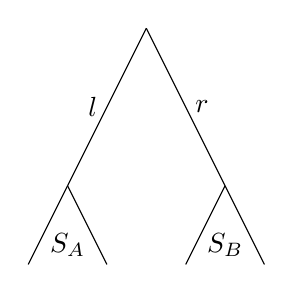
\begin{tikzpicture}
  \coordinate (P) at (0,2);
  \coordinate (A) at (-1.0,0);
  \coordinate (A1) at (-1.5,-1.0);
  \coordinate (A2) at (-0.5,-1.0);
  \coordinate (B) at (1,0);
  \coordinate (B1) at (0.50,-1.0);
  \coordinate (B2) at (1.5,-1.0);
  \node (SA) at (-1.0,-0.75) {$S_A$};
  \node (SB) at (1.0,-0.75) {$S_B$};
  \draw[] (P) -- node [left] {$l$} (A);
  \draw[] (P) -- node [right] {$r$} (B);
  \draw[] (A) -- (A1);
  \draw[] (A) -- (A2);
  \draw[] (B) -- (B1);
  \draw[] (B) -- (B2);
\end{tikzpicture}
\]

(weak coproduct diagram) %FIXME

extends to Weak Biproducts of arbitrary Set-indexed Families of Types
$\bigoplus_{i \in I} A_i$

In Process Calculus, these constructions yield \emph{Disjointly
  Guarded Sums}

Name-free, Names controlled indirectly via Types

applying general definition of Non-determinism and Semi-additivity
obtains $p + q = p \cup q$ which is the Interpretation of
Non-determinism in the Trace Model

in $\cat{ASProc}$ with Processes as Synchronization Trees Modulo Weak
Bisimulation, $p+q$ is a Non-associative version of CSP \emph{Internal
  Choice} $p \sqcap q$


\asterism


\textbf{Input/Output}

Type $X$:
\begin{align*}
  \Sigma_X &= \{\bullet\} \\
  S_X &= \Sigma_X^*
\end{align*}

Type $Y$ for an Input/Output pair Communicating with a single Client:
\begin{align*}
  \Sigma_Y &= \{inl(\bullet), inr(\bullet)\} \\
  S_Y &= a.b.S_Y + ab.S_Y
\end{align*}
where $a$, $b$, and $ab$ are abbreviations for $\{inl(\bullet)\}$,
$\{inr(\bullet)\}$, and $\{inl(\bullet),inr(\bullet)\}$, resp.
Compatible Clients are of the form $a.b.P$ where $P$ is the
Continuation Process.

\interrobang Note the above is inferred from the examples of Clients
given in \cite{abramsky-gay-nagarajan96}: $client = a.b.client$ and
$client = a.b.nil$

$cell : X \parr ... \parr X$

\fist Note unlike in $\cat{SProc}$, the Asynchronous Ports do not need
Delays ($\delta\Delta X$)


\textbf{Safety Specifications}

the above definition of $Y$ for an Input/Output pair Communicating
with a single Client has Deadlock Freedom

Example desired Safety Specification: ``Clients of a Scheduler are
Scheduled Cyclically''

$p : A$

Type $S$ with same Alphabet as $A$ but more restricted Safety
Specification

\emph{Safety Morphism} -- $s: A \rightarrow A$ such that $p : I
\rightarrow A$ Satisfies the Specification in $S$ if and only if $p =
s \circ p$

expresses stronger Specifications without ``forgetting'' what the
Interface looks like

for $s = \id_S$ (considered as a Morphism $A \rightarrow A$ because
$S_S \subseteq S_A$), $p = s \circ p \Leftrightarrow traces(p)
\subseteq S_S$

Correctness Proofs of Processes built from Subcomponents

(scheduler example)



% --------------------------------------------------------------------
\subsection{Proof Net} \label{sec:proof_net}
% --------------------------------------------------------------------

\cite{llwiki16}

Proof Nets can be seen as a Quotient of One-sided Sequent Calculus
Proofs (\S\ref{sec:sequent_calculus}) under Commutation of Rules



% --------------------------------------------------------------------
\subsection{Geometry of Synthesis} \label{sec:geometry_of_synthesis}
% --------------------------------------------------------------------

Bounded version of Geometry of Interaction



% --------------------------------------------------------------------
\subsection{Multiobject GOI}\label{sec:multiobject_goi}
% --------------------------------------------------------------------

\cite{haghverdi-scott05}

Multiplicative Linear Logic (\S\ref{sec:multiplicative_linear_logic})

Parital Trace (\S\ref{sec:partial_trace})
